\chapter{Results}
\label{results}

\section{Summary}

We present our results in three parts. 

In \autoref{validation}, we use \texttt{MorphCT} to test the performance of \texttt{pySCF} at the level of the chromophore.
Two experiments are reported. In the first, we calculate the frontier molecular orbital
energies for fused ring oligomers of increasing length. We compare the results of our experiment to the
results of the same experiment done with more rigerous DFT methods. In the second, we test the 
performance of the \texttt{pySCF} dimer calculations outlined in \autoref{methods}. 
We take two simple chromophores, two thiophene rings, in $5680$ oreintations and calculate the
electronic coupling between them. We do so to test if our dimer calculation correlates sensibly to the angle
and distance between chromophores. These experiments are broadly meant to confirm that we have integrated
\texttt{pySCF} into \texttt{MorphCT} properly, and that the quantities produced comport with the physics of these systems.
We then deploy \texttt{MorphCT} on three benchmark P3HT morphologies to obtain charge mobility
and compare the results to previously reported values for these morphologies. This section is meant to
validate the current implementation of \texttt{MorphCT} against a previous implementation. 

In \autoref{sensitivity}, we test the sensitivity of our \texttt{MorphCT} calculated mobilites to dcut, chromophore
reorganization energy, KMC temperature, and choice of charge carrier lifetimes for MSD analysis. Using a
benchmark P3HT morphology, holding all other parameters constant and sweeping accross relevant scales
provides context for how to treat these parameters in future investigations. 

In \autoref{itic}, we present the results of an investigation of ITIC from molecular structure to MD predicted
morphology to KMC predicted charge mobility. We use this opportunity to explore the TRUEness of
\texttt{MorphCT}. 

\section{Validation}

\label{validation}

\subsection{Quantum Chemical Calculation Validation}

As outlined in \autoref{qccmethods}, QCC is used in two distinct way in our workflow. 
First it is used to estimate free energy
difference between individual chromophores as the difference in their HOMO (or LUMO) energy levels.
Secondly, it is used to estimate the electronic overlap ($T_{ij}$) with the dimer splitting method which involves
calculating the HOMO(or LUMO) of the dimer formed by the two chromophores. We present the results from two
exploratory experiments meant to evaluate \texttt{pySCF}'s suitabilitity for performing these duties:
(1) we compare frontier molecular energies of single chromophores given by \texttt{pySCF} to those
given by more rigorous DFT and (2) we evaluate performance \texttt{pySCF}'s dimer calculation.

\subsubsection{Experiment 1 Methods}

At the level of a single chromophore, we calculate the HOMO-LUMO gap for fused-ring
oligomers of increasing length. 
The difference between the HOMO and LUMO energy levels, the HOMO-LUMO gap, is an approximation of the amount
of energy necessary to promote an electron to a higher energy level.  
Fused-ring geometries are of particular interest for accepter
molecules, as discussed for FREAs in the introduction. 
The fused thiophenes in this experiment represent a generic FREA core, whose frontier molecular oribitals are
the landing cites for a charge propigating through an acceptor material. 

To recreate these experiments, using \texttt{mBuild} \cite{Klein2016}, oligomers composed of 4-8 planar fused thiophene rings
were intialized and saved to a GSD file. The GSD files were fed into \texttt{MorphCT} which uses \texttt{pySCF} to quantify the
frontier orbital energy levels \autoref{qccmethods}.

\subsubsection{Experiment 1 Results}

Our values for the HOMO-LUMO gap are plotted by oligomer length in \autoref{fig:fused}. 
Our HOMO-LUMO gap ranges between $7.27eV$ and $6.34eV$. Consistent with our findings using a larger data set
in \autoref{itic}, the wall time for these individual calculations take place on the order of seconds. 

Furthermore, it is known that there is a near linear
relationship between HOMO-LUMO gap and oligomer length. We find that our use of \texttt{pySCF} (MINDO/3) replicates
this trend and this is clear from \autoref{fig:fused}.

As INDO methods are known to overestimate DFT values by a factor of 2-3 \cite{Gorelsky2001}, we find that our
implementation adequately recreated these results.
These results compare well to the values found using ab initio DFT were between $5.26eV$ and $4.92eV$. 
 those carried out with more rigorous DFT methods \cite{Arago2010}.

\begin{figure}
  \center
  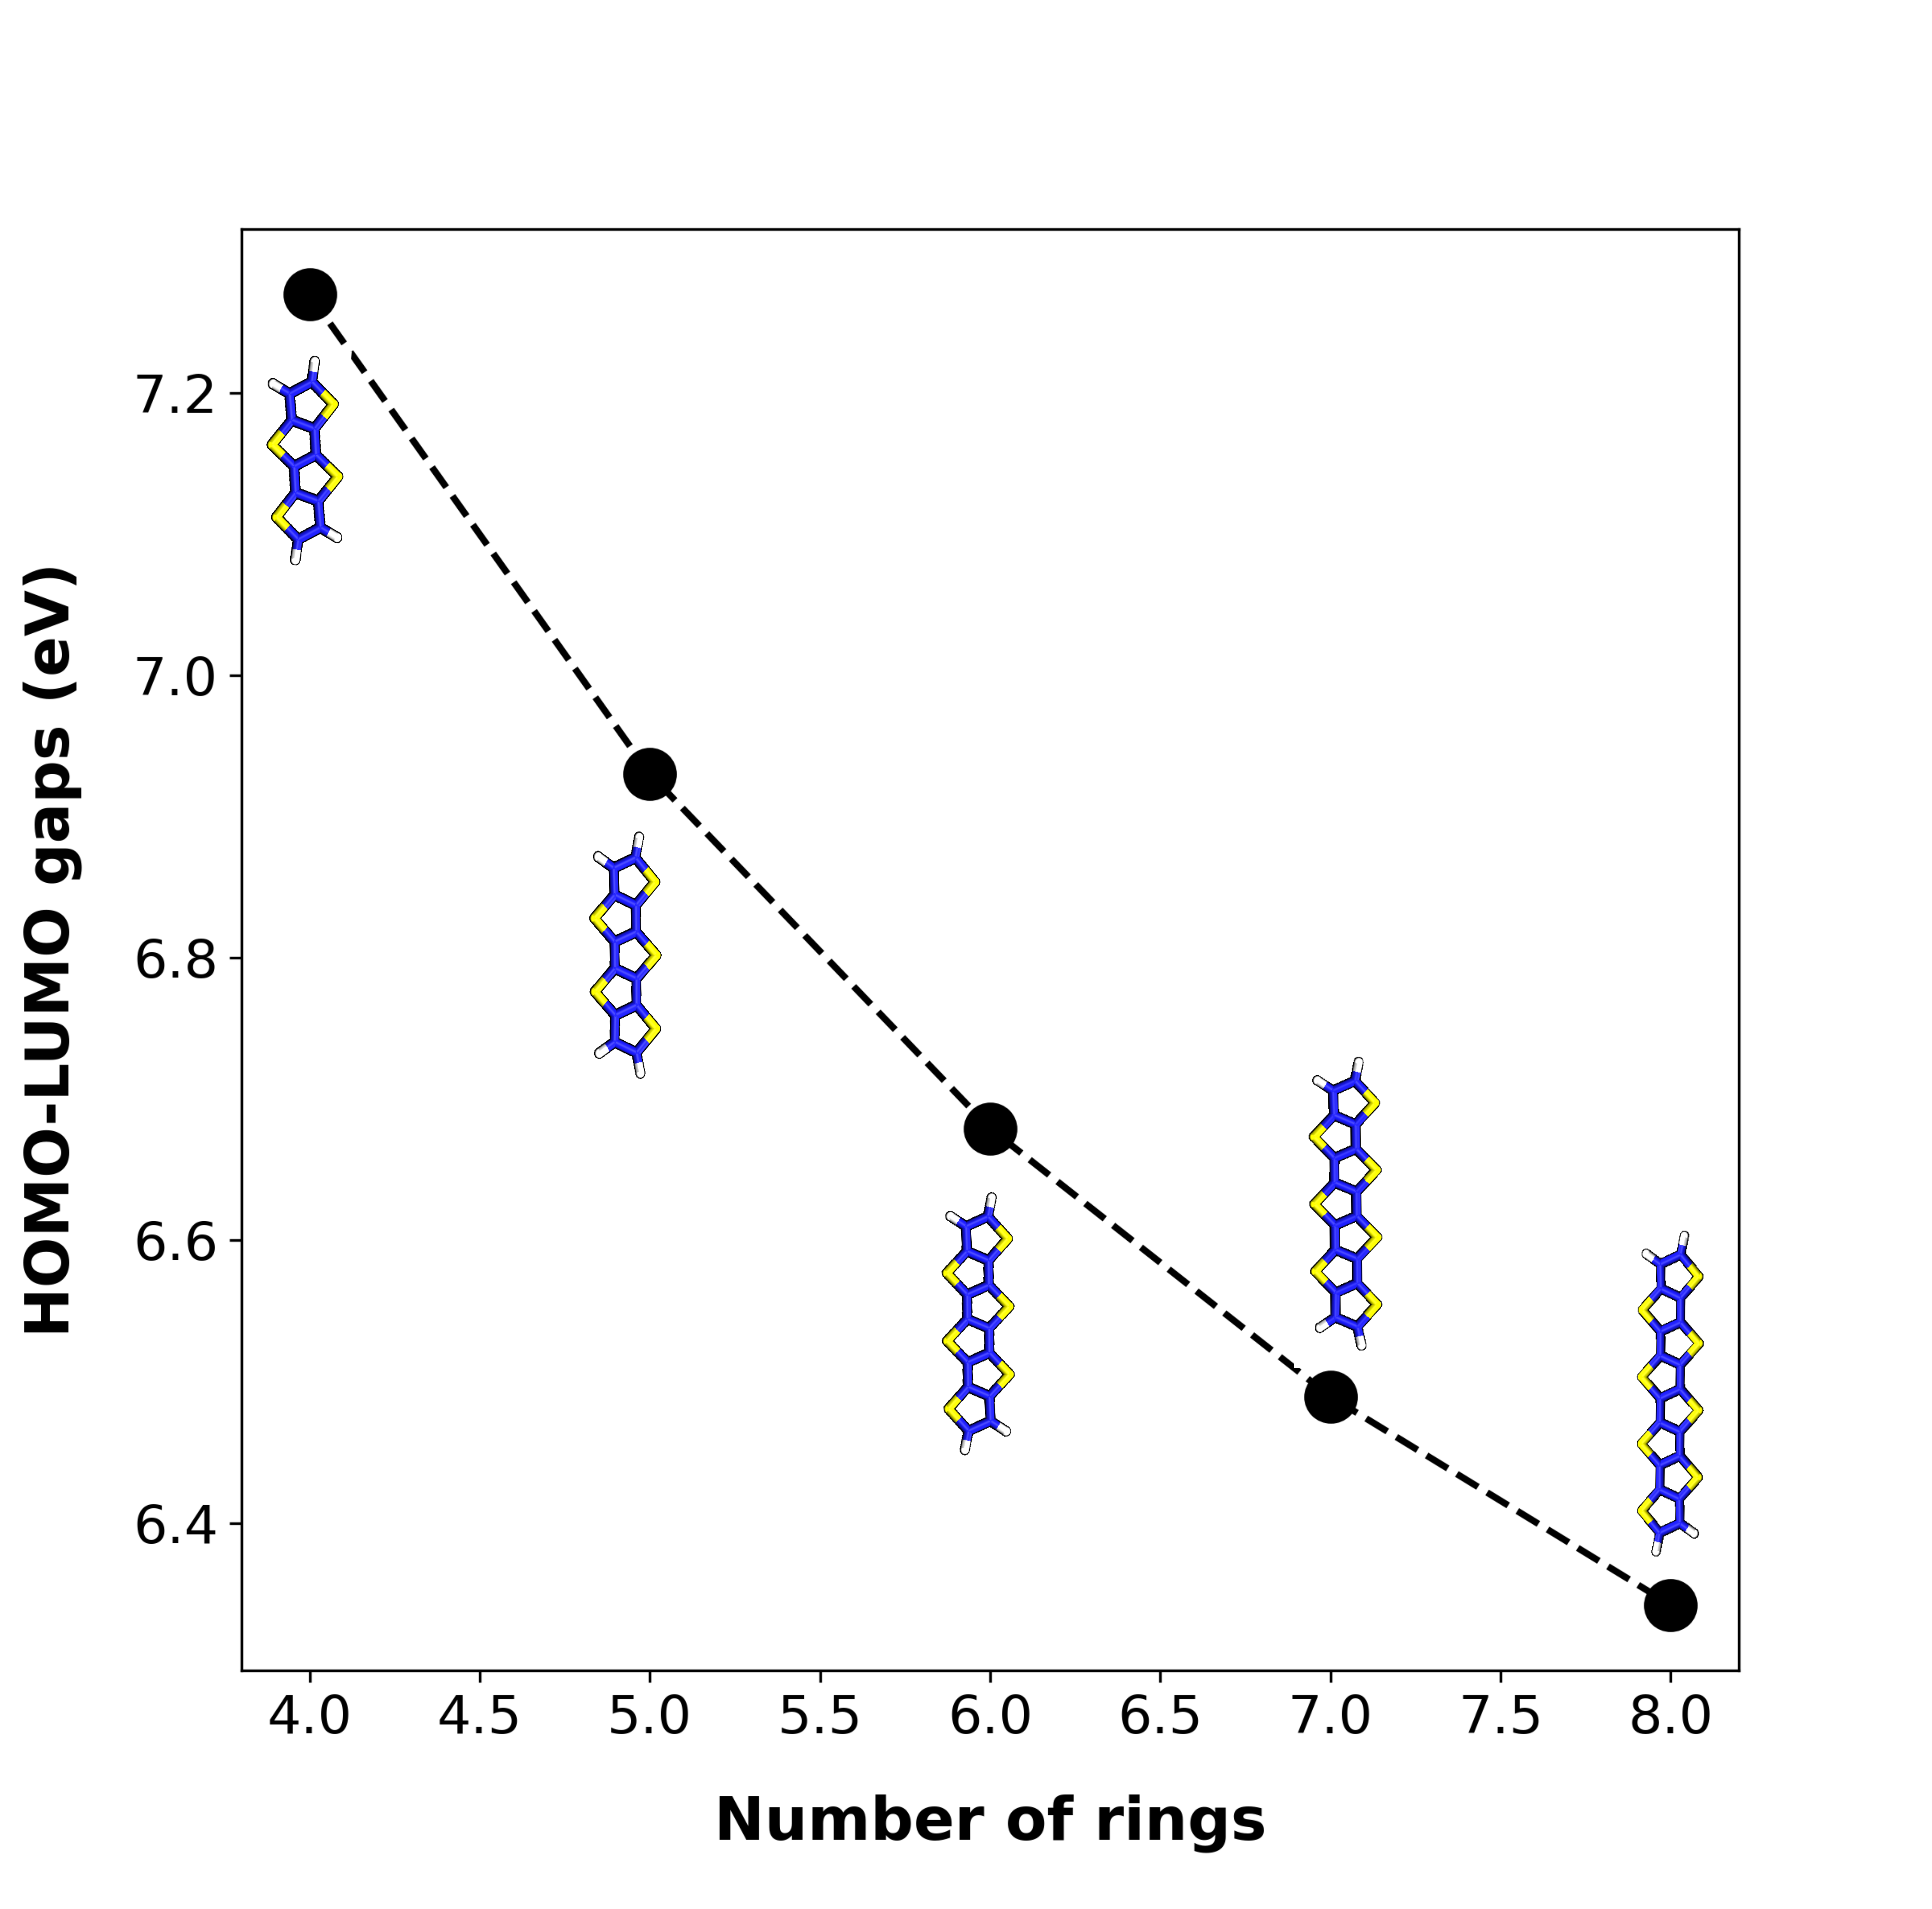
\includegraphics[width = .6\textwidth]{figures/fused-ring-figure.png}
  \caption{HOMO-LUMO gap obtained using \texttt{MorphCT} for fused-ring molecules of oligmer length $4-8$.}
  \label{fig:fused}
\end{figure}

\subsubsection{Experiment 2 Methods}

At the level of the chromophore pair, we explore the effect of angle and distance on the electronic orbital
overlap, $T_{ij}$, between two non-bonded thiophene rings.
Two thiophene rings are positioned in electronic proximity using \texttt{mBuild} and saved to gsd. 

A reference thiophene was placed at the origin in the xy-plane
with the y-axis running through the sulfur atom as shown in \autoref{TIplots}(a). For the second thiophene,
two sets of 12 rotations about the x-axis and z-axis (with $- \frac{\pi}{2} < \theta< \frac{\pi}{2}$)
and two sets of 12 translations bewteen $0nm$ and $0.5nm$ along the x-axis and z-axis were defined.
The cartesian product of these sets define a space of $12^{4}= 20736$ oreintations for second thiophene. 

Oreintations resulting in atoms that were less
than $0.3nm$ were removed from the data set as distances shorter than this are considered
unphysical. The remaining $5680$ atomic arrangements were saved to a GSD and the $T_{ij}$ was quantified for
each with \texttt{MorphCT}. 

\subsubsection{Experiment 2 Results}

The data resulting from this experiment, $5680$ oreintations of electronically 
interacting non-nonded thiophenes and the
correspinding $T_{ij}$ between them, provide evidence that \texttt{MorphCT} is rationally capturing the orbital
overlap between chromophores. 
The $T_{ij}$ resulting from these $5680$ orientations are shown in \autoref{TIplots}. 
The figure shows that, as expected, a decrease in 
center-to-center distance results in more orbital overlap and thus an increase in $T_{ij}$. 
Also observable in the figure is that
a negative rotation about the x-axis orients the sulfer downward, resulting in a smaller sulfer-to-sulfler distance 
and a greater $T_{ij}$. 

\begin{figure}
\centering
\begin{subfigure}{.9\textwidth}
    \centering
    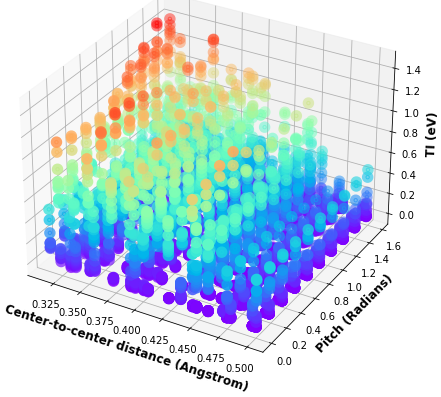
\includegraphics[width=\textwidth]{figures/transfer_integral_plot.png}
    \caption{Individual dots correspond to $5680$ 
    distinct combinations of rotations and translations of the upper
    thiophene.
    Dots are colored based on the $T_{ij}$ between thiophenes for the given x-axis rotation,
    z-axis rotation, and center to
    center distance from the reference thiophene.}
\end{subfigure}
\\
\begin{subfigure}{.5\textwidth}
    \centering
    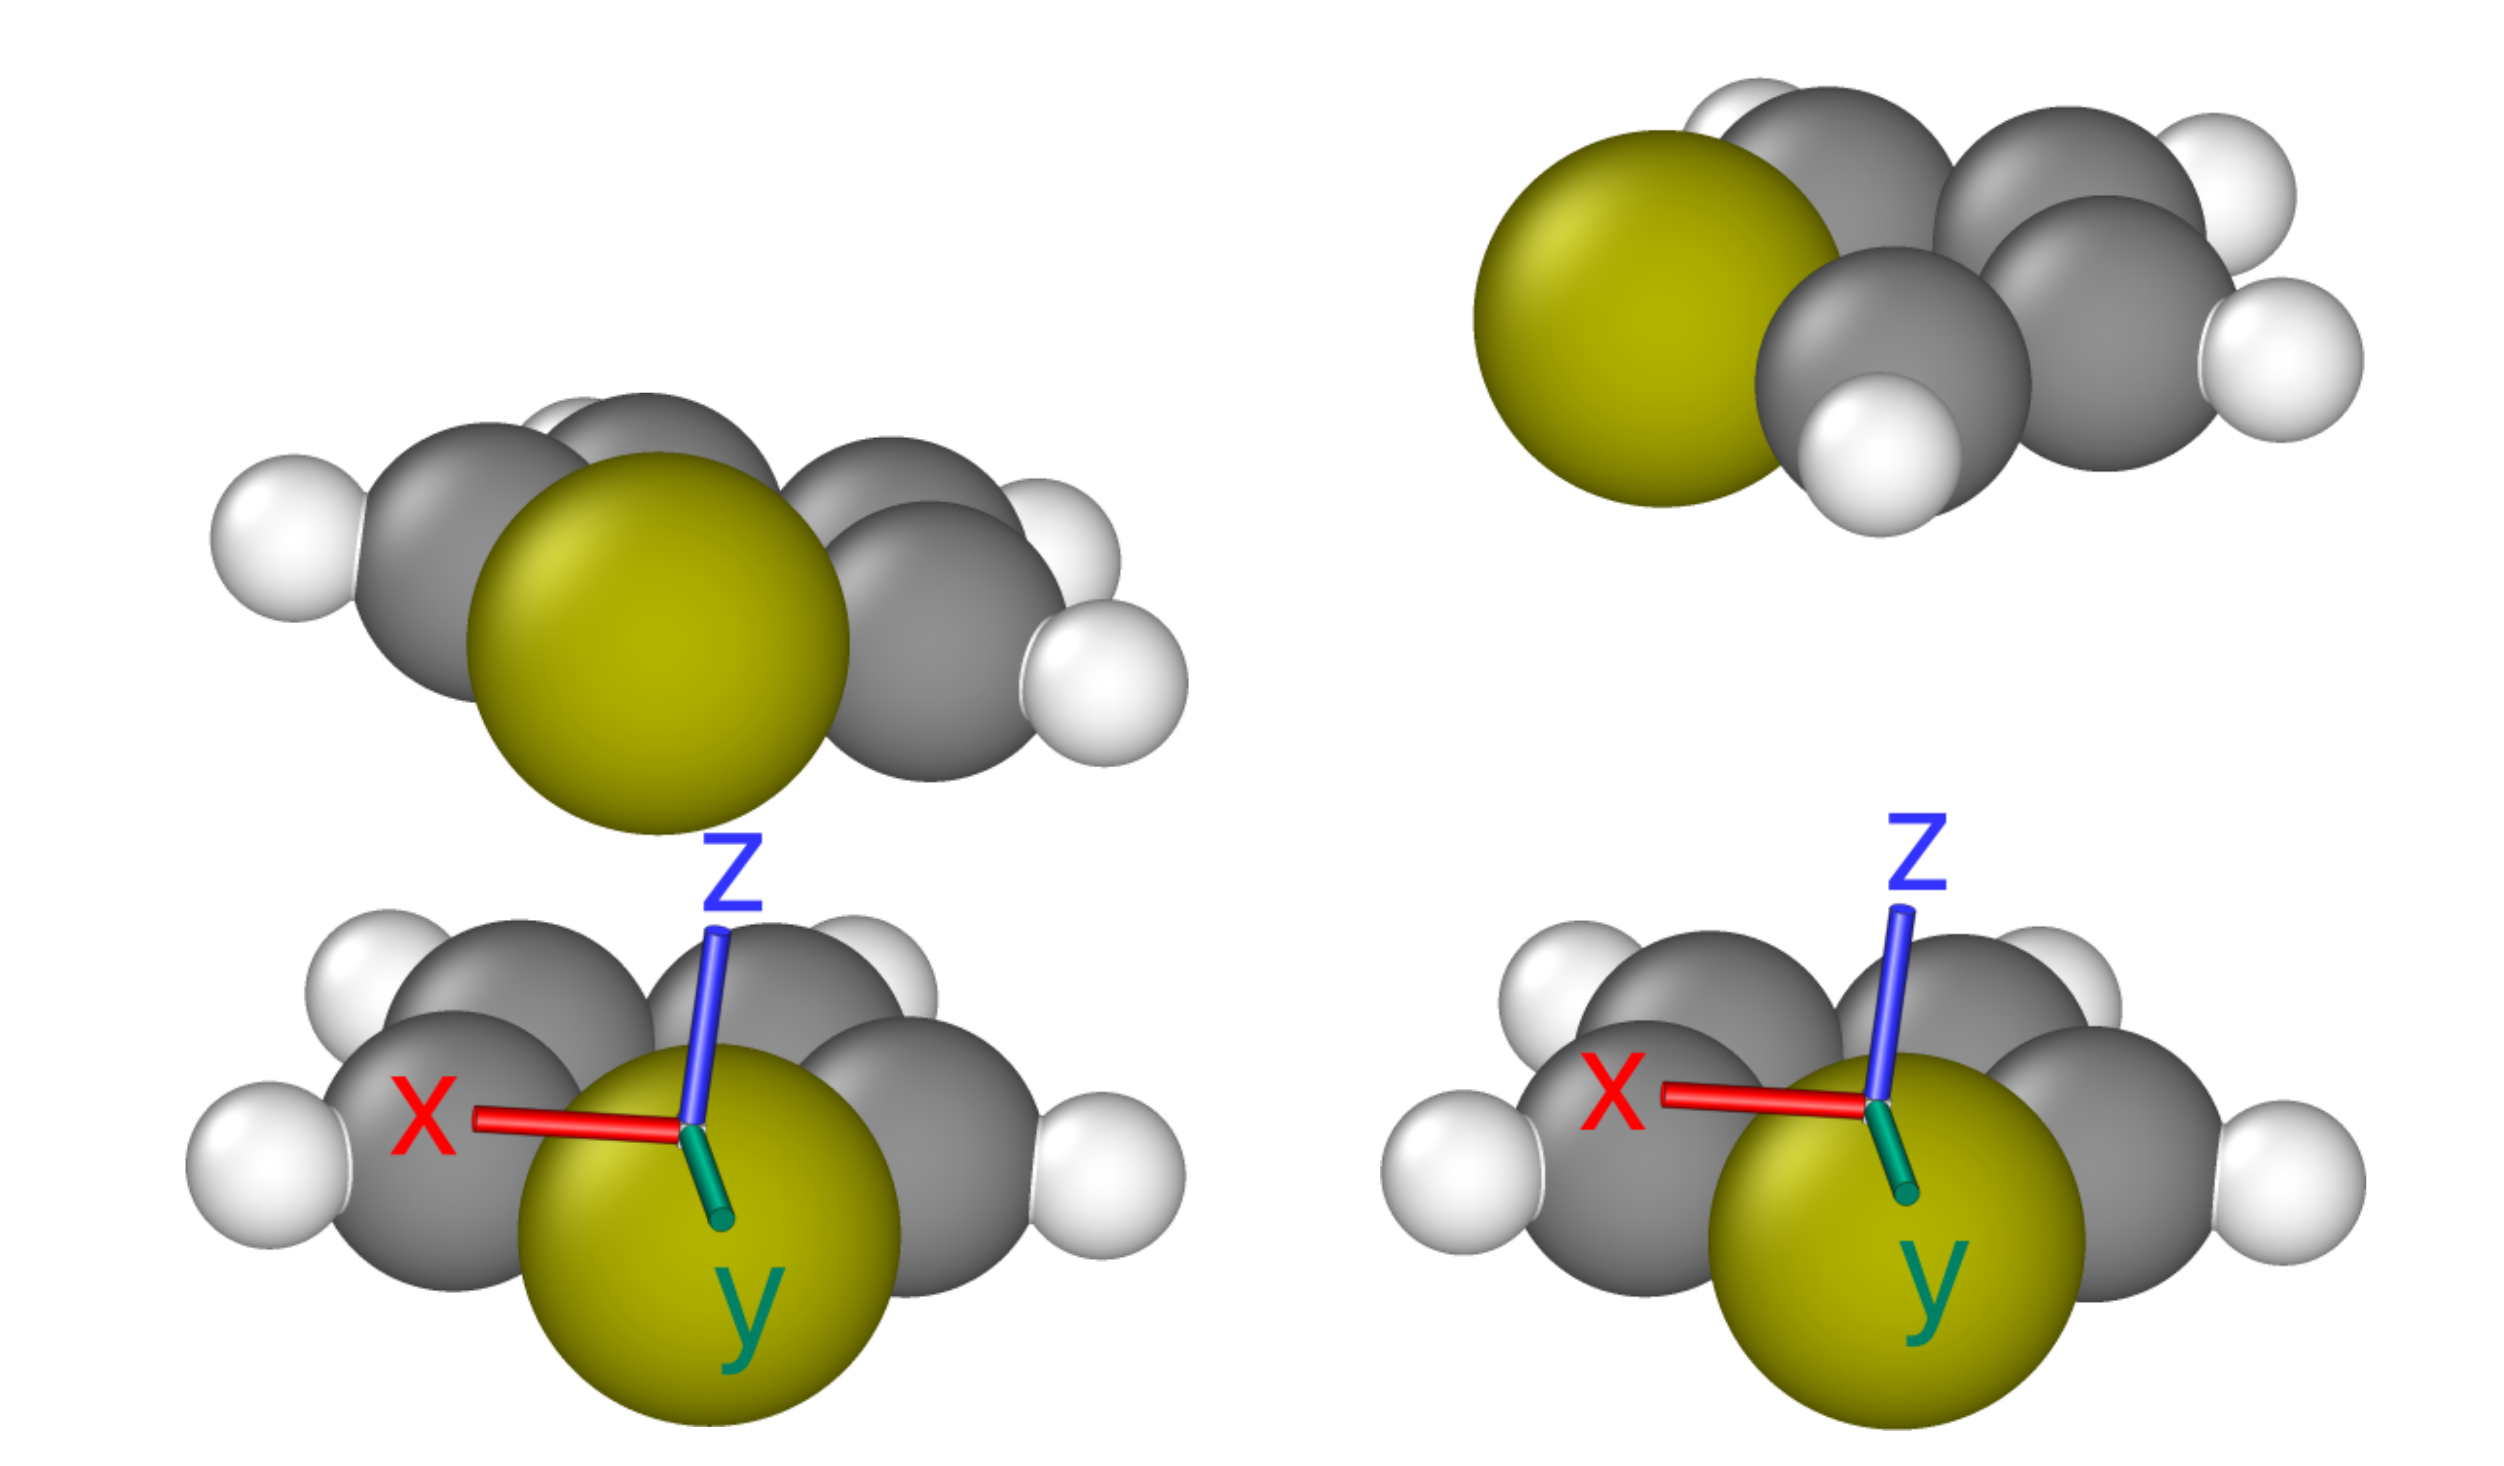
\includegraphics[width=\textwidth]{figures/thiophene-oreintations.png}
    \caption{The orientation with the hightest $T_{ij}$ on the left and
    the lowest on the right.}
\end{subfigure}%
\caption{ }
\label{TIplots}
\end{figure}

For the oreintations found to be most and least optimal we calculate (shown in \autoref{TIplots}),
a $T_{ij}$ of $.00005eV$ and $.15eV$ respectively. In the context of \autoref{marcus} and \autoref{waittime},
the corresponding wait time for a charge to hop between to thiophenes in these oreintations is $\tau = 2
\cdot 10^{-14}s$ and $\tau = 2 \cdot 10^{-7}s$. With latter case being two orders of magnitude slower than the
lifetimes allowed in our KMC simulations, a hop would be highly unfavored for this oreintation. 

Creating the directory of GSDs and quantifying the $T_{ij}$ between them took a wall time of $3.2h$ which
avereges to ${\sim}2s$ per oreintation. 

As evidenced by \autoref{TIplots}((a)), for oreintations resulting in a center-to-center distance of less than
$0.5nm$ we calculate an average $T_{ij}$ of ${\sim} 0.28eV$.  
These calculations match closely those
calculated using more rigerous ab initio DFT methods\cite{Lan2008},
where realistic distances between thiophene rings in lamaeler P3HT crystals 
between $0.38nm$ and $0.4 nm$ gives $T_{ij}$ values between $0.07eV$ and $0.1eV$. 

In a similar work using a random forest machine learning to predict $T_{ij}$
between thiophenes based on 9 input features, the authors found that the
features of most importance for predicting $T_{ij}$ was bonded vs non bonded,
center-to-center distance and rotation about the y-axis. \cite{Jankowski2019c}

Graduating these pairwise energetics to charge characteristics on the scale of MD simulations
requires the use of an iterative algorithm. For this we employ KMC simulations using \texttt{MorphCT}.

\subsection{Charge Transport Calculation Validation}

Having explored the performance of \texttt{pySCF} on the level of the molecule, we graduate these computations to the
macroscopic scale with \texttt{MorphCT} to obtain charge mobility.
In a previous work \cite{Miller2018}, researchers used \texttt{MorphCT} to predict charge mobility in P3HT. 
With \texttt{pySCF} newly integrated into \texttt{MorphCT} for reasons outlined in \autoref{morphct},
we validate our charge mobility against this work.
The benchmark morphologies, which are the final frame of benchmark MD simulations,
used to carry out this validation are public \cite{P3HTData}. 

These benchmark simulations were carried out using coarse-graining techniques
wherein molecular segments have been unified and treated as individual beads to lower
computational cost and allow for larger and longer simulations. 
Using the Optimized Potentials for Liquid Simulations United Atom (OPLS-UA) force field,
the researchers ran united-atom simulations, which do
not explicitly keep track of the hydrogens in the simulation, 
but nevertheless accurately predict equilibrium geometries. This allowed the researchers to access length scales
at which individual grains can form within the morphology. The orientation and boundaries of these grains effect
charge transport and therefore provide a critical benchmark to compare against. 

We first fined-grained MD data (hydrogens appended back into
the morphology) and converted from .xml to .gsd format. At current, \texttt{MorphCT} is compatable with all atom data
and .gsd format. As visualized in \autoref{molecules}, chromophores are taken to be individual monomers. 
Using \texttt{MorphCT}, for each chromophore, a unique object is instantiated and the energetics are obtained using
\texttt{pySCF}. A KMC simulation is performed on the basis of these energetics with KMC temperature set to 300K. For
each morphology, 10,000 individual charge carriers are injected (one at a time) into the morphology, with
5,000 restricted to a lifetime of a tenth of a nanosecoond and 5,000 restricted to a liftime of a nanosecond.
As outlined in \autoref{kmcanalysis}, from the difference in MSD bewteeen these sets of charge carriers the
zero-field charge mobility for the morphology is obtained. 

\begin{figure}
  \center
  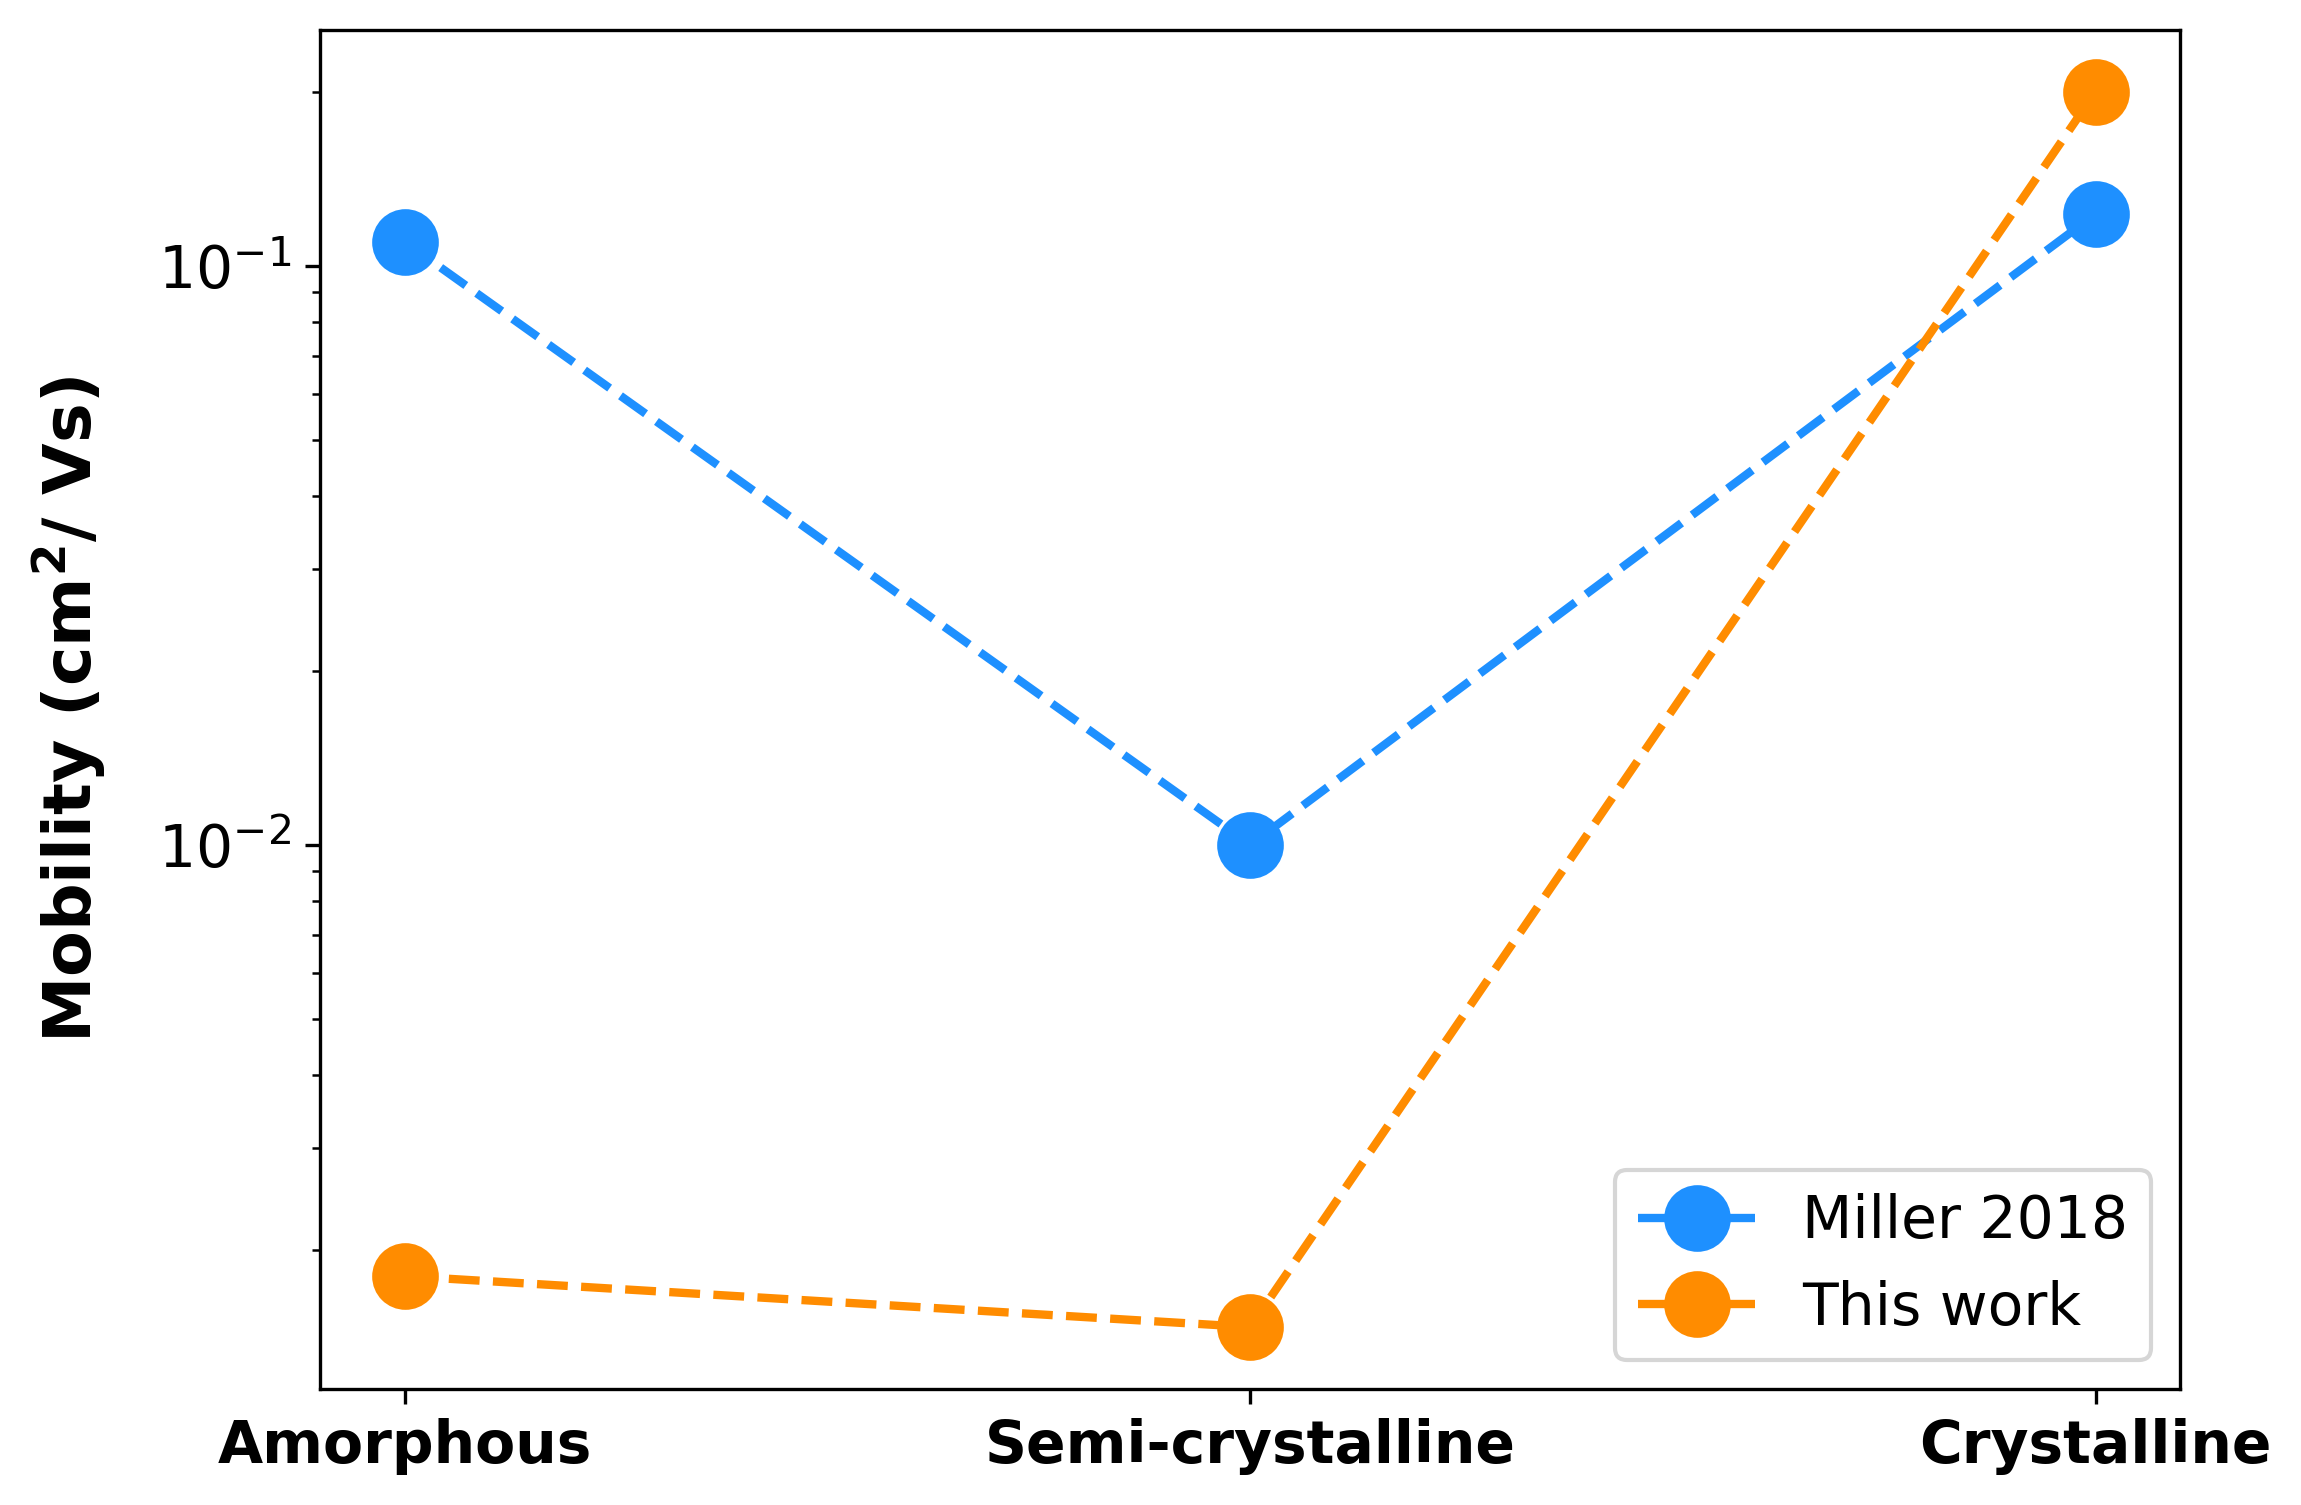
\includegraphics[width = .6\textwidth]{figures/validation.png}
  \caption{}
  \label{mobility-validation}
\end{figure}

It is known about P3HT that it can have vastly different crystallinities based on how it has been processed. 
We validate on three morpholgies with crystallinities that vary from amorphous to highly crystalline. These morphologies have been coerced into various levels of crystallinity through a simulated anhealing process. 
We refer to these morphologies as disordered, semi-crystalline, and crystalline.

Results from our work compare well to a predecessor of our work, which implemented ZINDO/s, another
semi-empirical QCC method \cite{Miller2018a}\cite{jones2017}. 
Their work utilized an earlier version of \texttt{MorphCT} which used the QCC software 
ORCA \cite{Neese2012b} to provide the quantum chemical approximations. 
ORCA's proprietary licensing was prohibitive in the efforts to containerize \texttt{MorphCT} for use on cluster and for
creating reproducible results. This motivated the restructuring of \texttt{MorphCT} for use with \texttt{pySCF}. The
performance of \texttt{pySCF} and of the current \texttt{MorphCT} workflow is the subject \autoref{results}.

The results in \ref{table:nonlin} show the charge mobility reported in the prior work, which used ORCA for
the QCC calculation, and the charge mobility obtained using using the current workflow, which uses \texttt{pySCF}. 
The previous work found that charge mobility is highest for the crystalline morphology, followed by the
amorphous, and finally the semicrystalline. This seemingly anomolous behavoir can be explained. While the
semicrystalline morphology has more ordered high speed highways of transport, the anisotropic movement
inhibits average displacement. 

Our work replicates this trend. However, the absolute value of charge mobility is only an order of magnitude
match for the crystalline morphology. 

\section{Charge Transport Sensitivity Analysis}

\label{sensitivity}

The sensitivity of our charge mobility calculations to various parameters was performed on the benchmark 
crystalline P3HT morphology. As the overarching goal is to connect the morphological features to charge
mobility, it is critical to be explicit about how each parameter can proscribe the resulting value of charge
mobility. Sensitivty analysis of this type can help us understand where to invest recources into dialing
the accuracy of any given parameter. It also gives motivation to be meticulous about keeping these parameters
consant accross analysis of the same material under different processing conditions. For example, if a higher
charge mobility is discovered for a given morphology after some simulated annhealing,
it should be confirmed that it is not because the researcher used a lower reorganization energy for example. 
[section needs work]


\subsection{Neighbor Cutoff (dcut)}
\label{dcutresults}
Voronoi analysis allows for the computationally efficient partitioning of space into
polyhedra chromophore cells. As shown in \ref{fig:dcut}, chromophore $i$ is the neighbor of chromophore $j$
if the voronoi cells constructed around their geometric center
share a boundary with one another. 

With each chromophore pair requiring a relatively costly QCC, after narrowing down the chromophore pairs with voronoi, it
could be
computationally preferable to calculate the distances between all pairs and remove neighbors more than dcut
apart.

\begin{table}
\caption{Dcut Sensitivity}
\centering % used for centering table
\begin{tabular}{c c c c c c c c} % centered columns (4 columns)
\hline\hline %inserts double horizontal lines
    dcut $\text{\AA}$ & 4 & 6 & 8 & 10 & 12 & 14 & 16 \\ [0.5ex] % inserts table
%heading
\hline  % inserts single horizontal line
pairs & 318 & 22000 & 49000 & 96000 & 113026 & 113315 & 113315 \\ [1ex]% inserting body of the table
$\mu_{0}$ $(cm^{2}/Vs)$ & $-2.17 \cdot 10^{-6}$ & $6.13 \cdot 10^{-4}$ & .01 & .17 & .17 & .22 & .22 \\ [1ex] % [1ex] adds vertical space
%$\mu_{0}$ Error & $-1.75*10^{-6}$ & 6 & 8 & 10 & 12 & 14 & 16 \\
\hline %inserts single line
\end{tabular}
\label{table:dcut-sense} % is used to refer this table in the text
\end{table}

\autoref{table:dcut-sense} shows the effect of cutoff distance on value of
calculated mobility.  
 We can see in table \ref{table:dcut-sense}, that with dcut = 10 we get comparable mobilities to the
dcut 12 simulation with $10^5$ less
pairs, which could suggest that beyond dcut 10 there is a diminishing returns on mobility prediction with the
additional chromophores. 

However, we found for the materials currently under investigation,
\texttt{pySCF} is speedy enough such that intrucing dcut adds more ambiguity
into the workflow than is necessary given that the average time per QCC dimer calculation is .036s for P3HT and
1.2s for ITIC. Furthermore, with \texttt{MorphCT} acting on static atomistic oreintations, these calculations 
are only necessarily performed once per morphology. With that, our workflow defaults this cutoff distance to half
the length of the simulation box, rendering it effectively moot. 

If, in the future, more computationally expensive methods are incorperated into the QCC step, or chromophores in other
organic materials are a heavier lift \texttt{pySCF}, it could be benificial to reintroduce this cutoff distance. The optimal dcut will vary depending on the material and before doing large sweeping analysis on a new
material its at a discount to do some preliminary analysis to determine an apporiate value. We tested the
sensitivity of the algorithm to the value (dcut). 

\subsection{Reorganization energy}

In the context of \autoref{marcusmodel}, 
reorganization energy, $\lambda_{ij}$, constitutes the energy required to distort the dimer's equilibrium geometry with a
charge on chromophore $i$ into the dimers equillibrium geometry with charge on chromophore $j$.
Reorganization energy consist of the energy change associated with the destortion of the dimers geometry,
and the distortion of the surrounding medium in responce the movement of the charge. It can be written as
follows:
\begin{align}
    \lambda_{total} = \lambda_{internal} + \lambda_{external}.
\end{align} 
$\lambda = 0.3eV$ is chosen to be the default reorganization energy ($\lambda_{internal} = 0.1eV$
and $\lambda_{external} = .02eV$) as others have done with P3HT \cite{jones2017} and
a flourene-triphenylamine copolymer, TFB \cite{Gali2017}. 

\begin{figure}
\centering
\begin{subfigure}{\textwidth}
    \textbf{(A)} \\
    \centering
    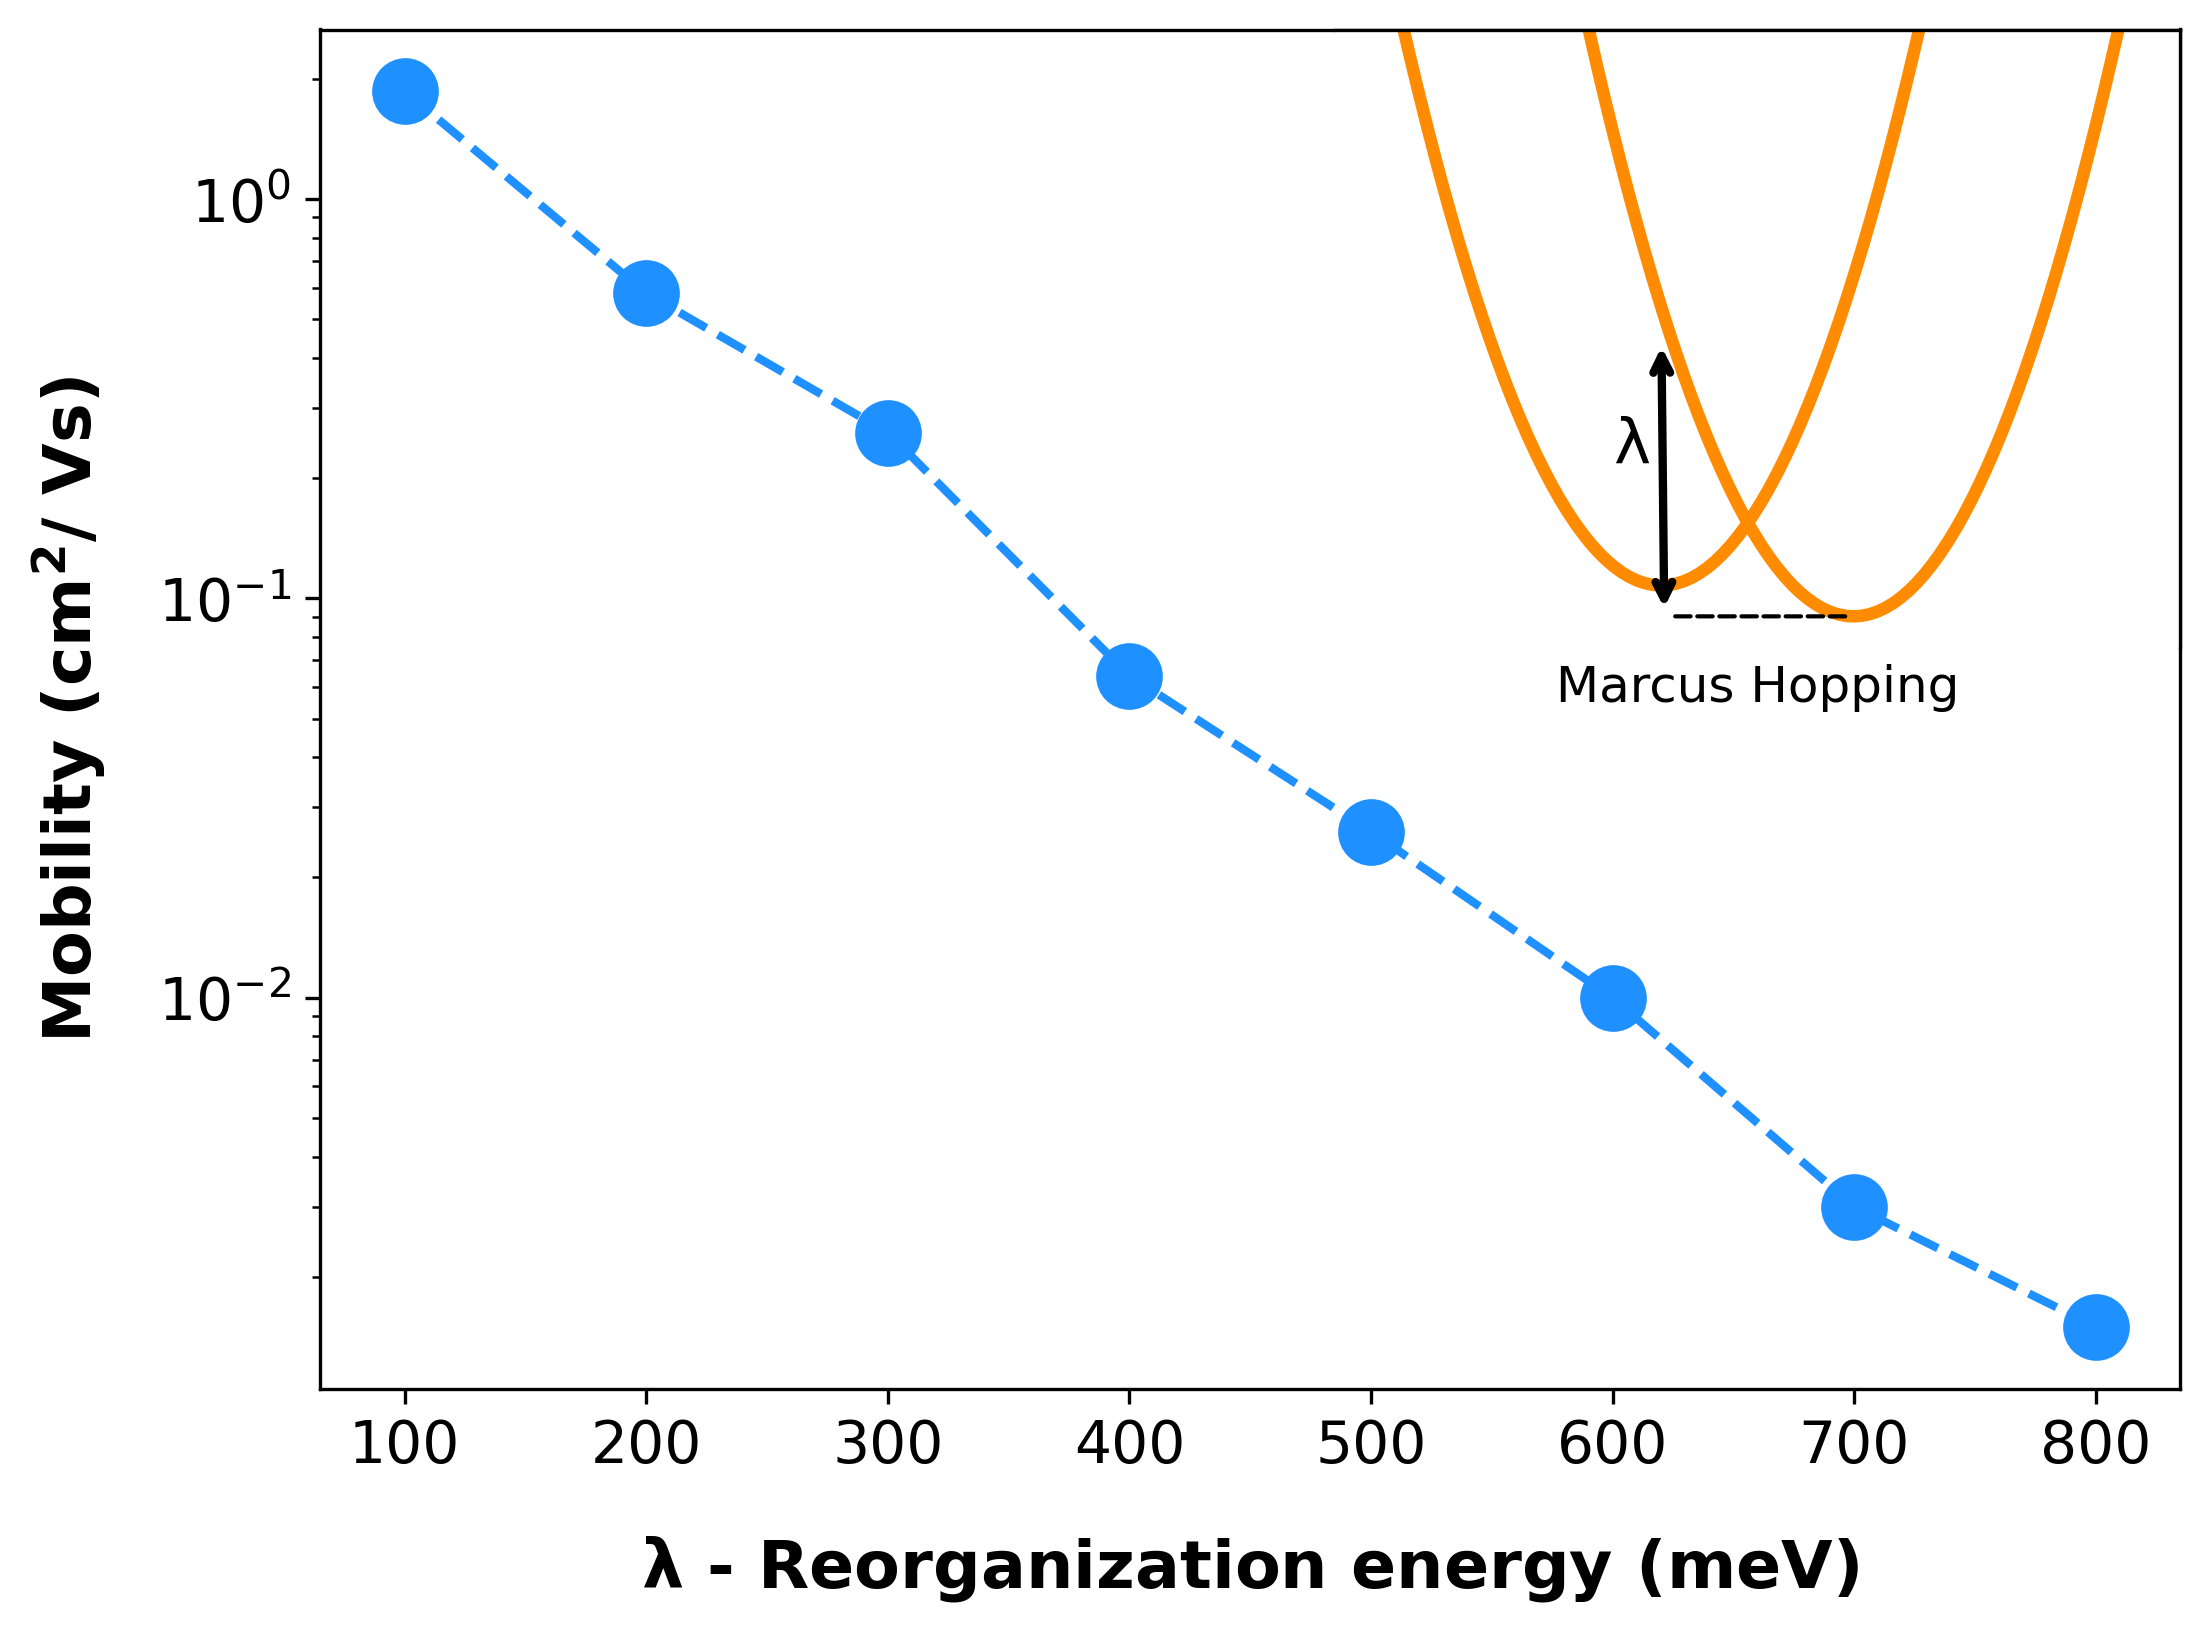
\includegraphics[width=.8\textwidth]{figures/reorg-log-yaxis.png}
    \newline
\end{subfigure}%
\\
\begin{subfigure}{.5\textwidth}
    \textbf{(B)} $\lambda = 100$
    \centering
    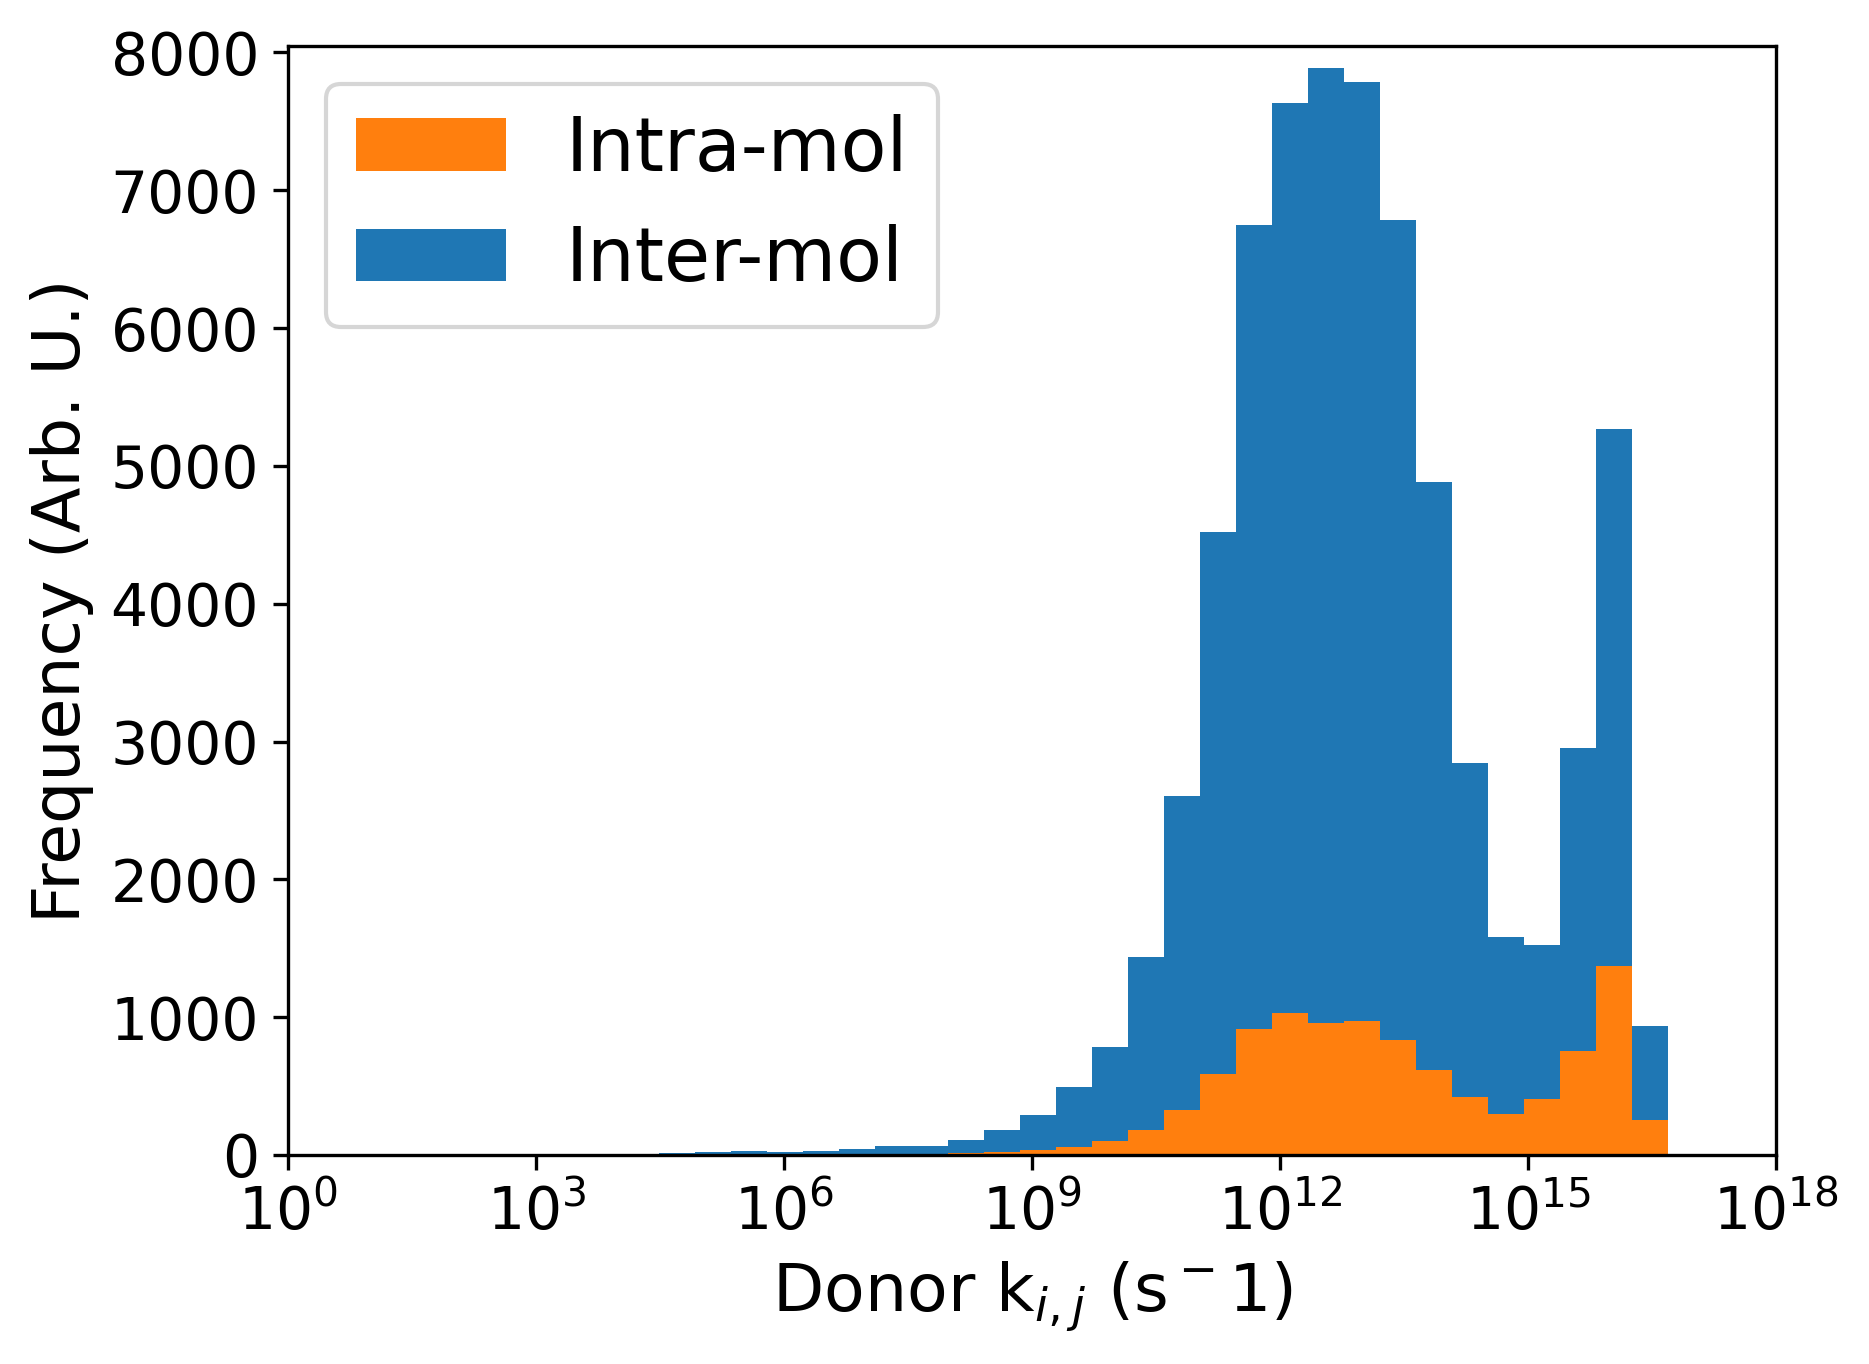
\includegraphics[width=\textwidth]{figures/donor_hopping_rate_clusters_reorg100.png}
\end{subfigure}%
\begin{subfigure}{.5\textwidth}
    \textbf{(C)} $\lambda = 800$
    \centering
    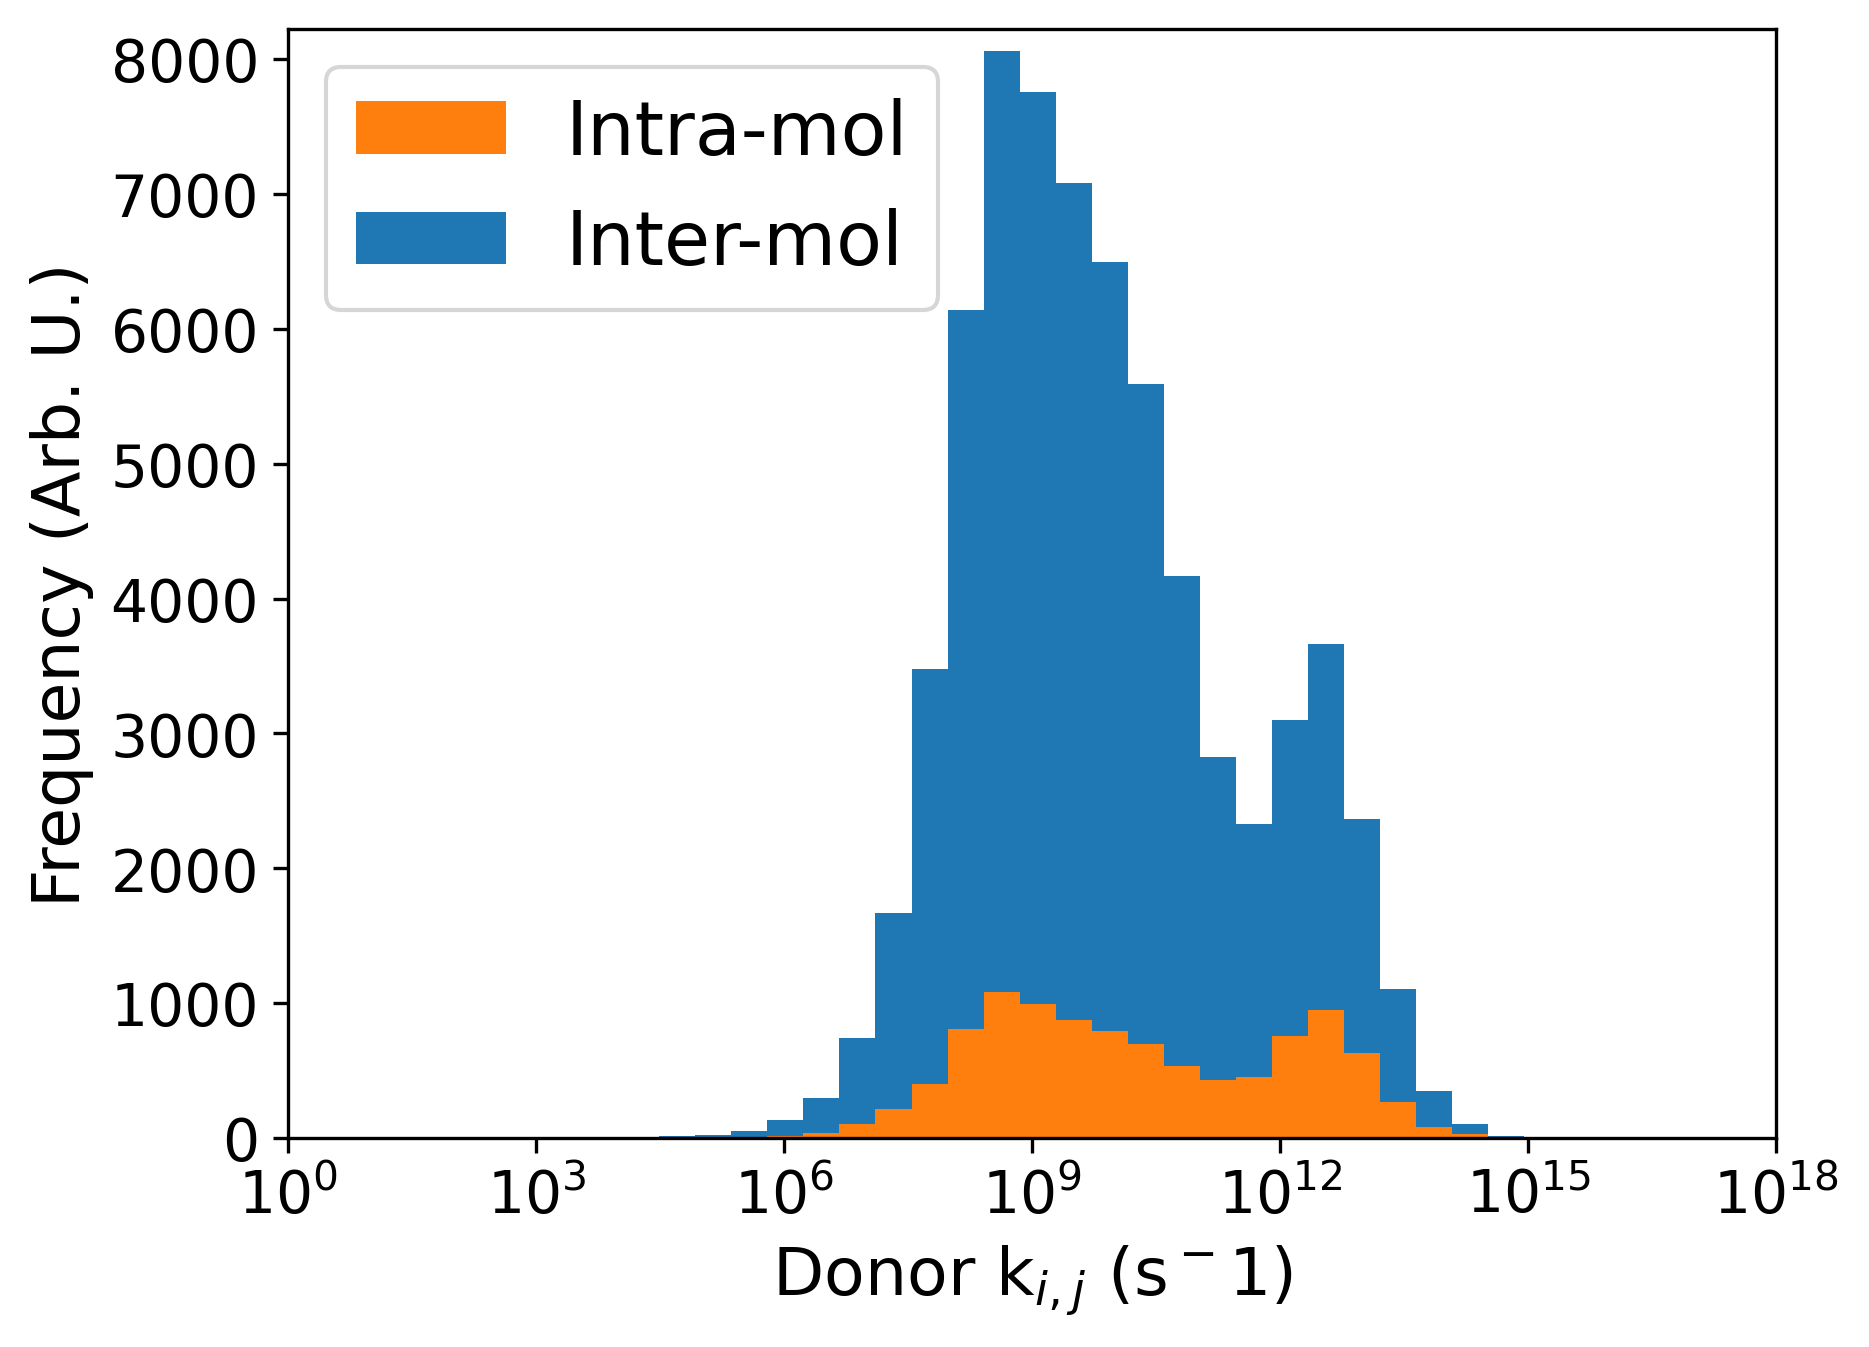
\includegraphics[width=\textwidth]{figures/donor_hopping_rate_clusters_reorg800.png}
\end{subfigure}
    \caption[short]{Figure (A) shows how KMC simulated mobility values scale with the perscribed
    reorganization energy values, $\lambda$. Figures (B) and (C) show the distrubtion of hopping rates with
    $\lambda = 100eV$ and $\lambda = 800eV$ respectively. These show how $\lambda$ effects the in the Marcus
    rate accros the morphology and thus the charge mobiility.}
\label{reorg}
\end{figure}

Reorganization energy has a strong effect on charge mobility in organic
molecules[REFS]. In our workflow, reorganization energy is set as an attribute
to the chomophore object. It is defaulted to $~300meV$ as for all chromophore
objects.

To test the sensitivity of the algorithm to this value we ran 8
simulations with chromophores assigned reorganization energies of 100-800meV. The results, shown in
\autoref{reorg}, are expected from the inspection of \autoref{marcus}. Because these simulation were run on
the same morphology, the variation in distributions of $k_{ij}$ values, shown in \autoref{reorg}(B)(C), is
solely due to the choice of $\lambda$. The cumulative outcome of this is the exponetial decay in mobility as
$\lambda$ is increased.

\subsection{Temperature}

Another parameter of interest in the Marcus theory mention above is temperature. To test the sensitivity to
temperature, 15 KMC simulations from 100K to 800k were run on the benchmark P3HT crystalline morphology. It
is clear from the results in figure \ref{TEMP}(A) that the mobilities trend upward with temperature. With relatively
weak electronic coupling ($T_{ij}$) between chromophores, electron transfer proceeds nonadiabatically
\cite{clarke2010}. With this weak coupling, the temperature in the Gibbs free energy of activation term
dominates the effect temperature has hop rate.

An unanticipated result is that increasing the temperature of the KMC
simulation also increases the wall time that the simulations required to
complete. As an illustration of why this is the case, the distribution of hop
rates is plotted for 100K and 800K in figure \ref{TEMP}(C)(D). With the distribution of hop rates skewed
drastically higher at 800K, each charge carrier will experience orders of
magnitude more hops during its specified lifetime. 

If extremely cold
temperatures are to be investigates in the future, thought should probably be given to
the decreasing contribution to statistical significance from the addition of
any single charge carrier. 

\begin{figure}
\centering
\begin{subfigure}{.5\textwidth}
    \textbf{(A)}
    \centering
    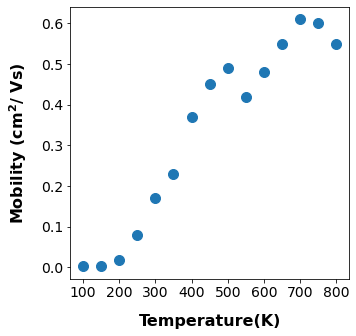
\includegraphics[width=\textwidth]{figures/temp.png}
    \newline
\end{subfigure}%
\begin{subfigure}{.5\textwidth}
    \textbf{(B)}
    \centering
    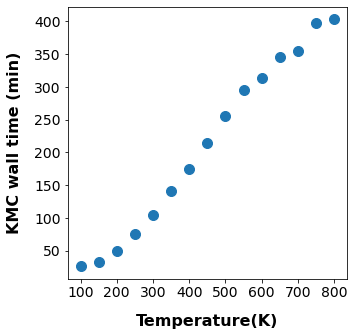
\includegraphics[width=\textwidth]{figures/temp_simtime_plot.png}
    \newline
\end{subfigure}
\begin{subfigure}{.5\textwidth}
    \textbf{(C) 100K}
    \centering
    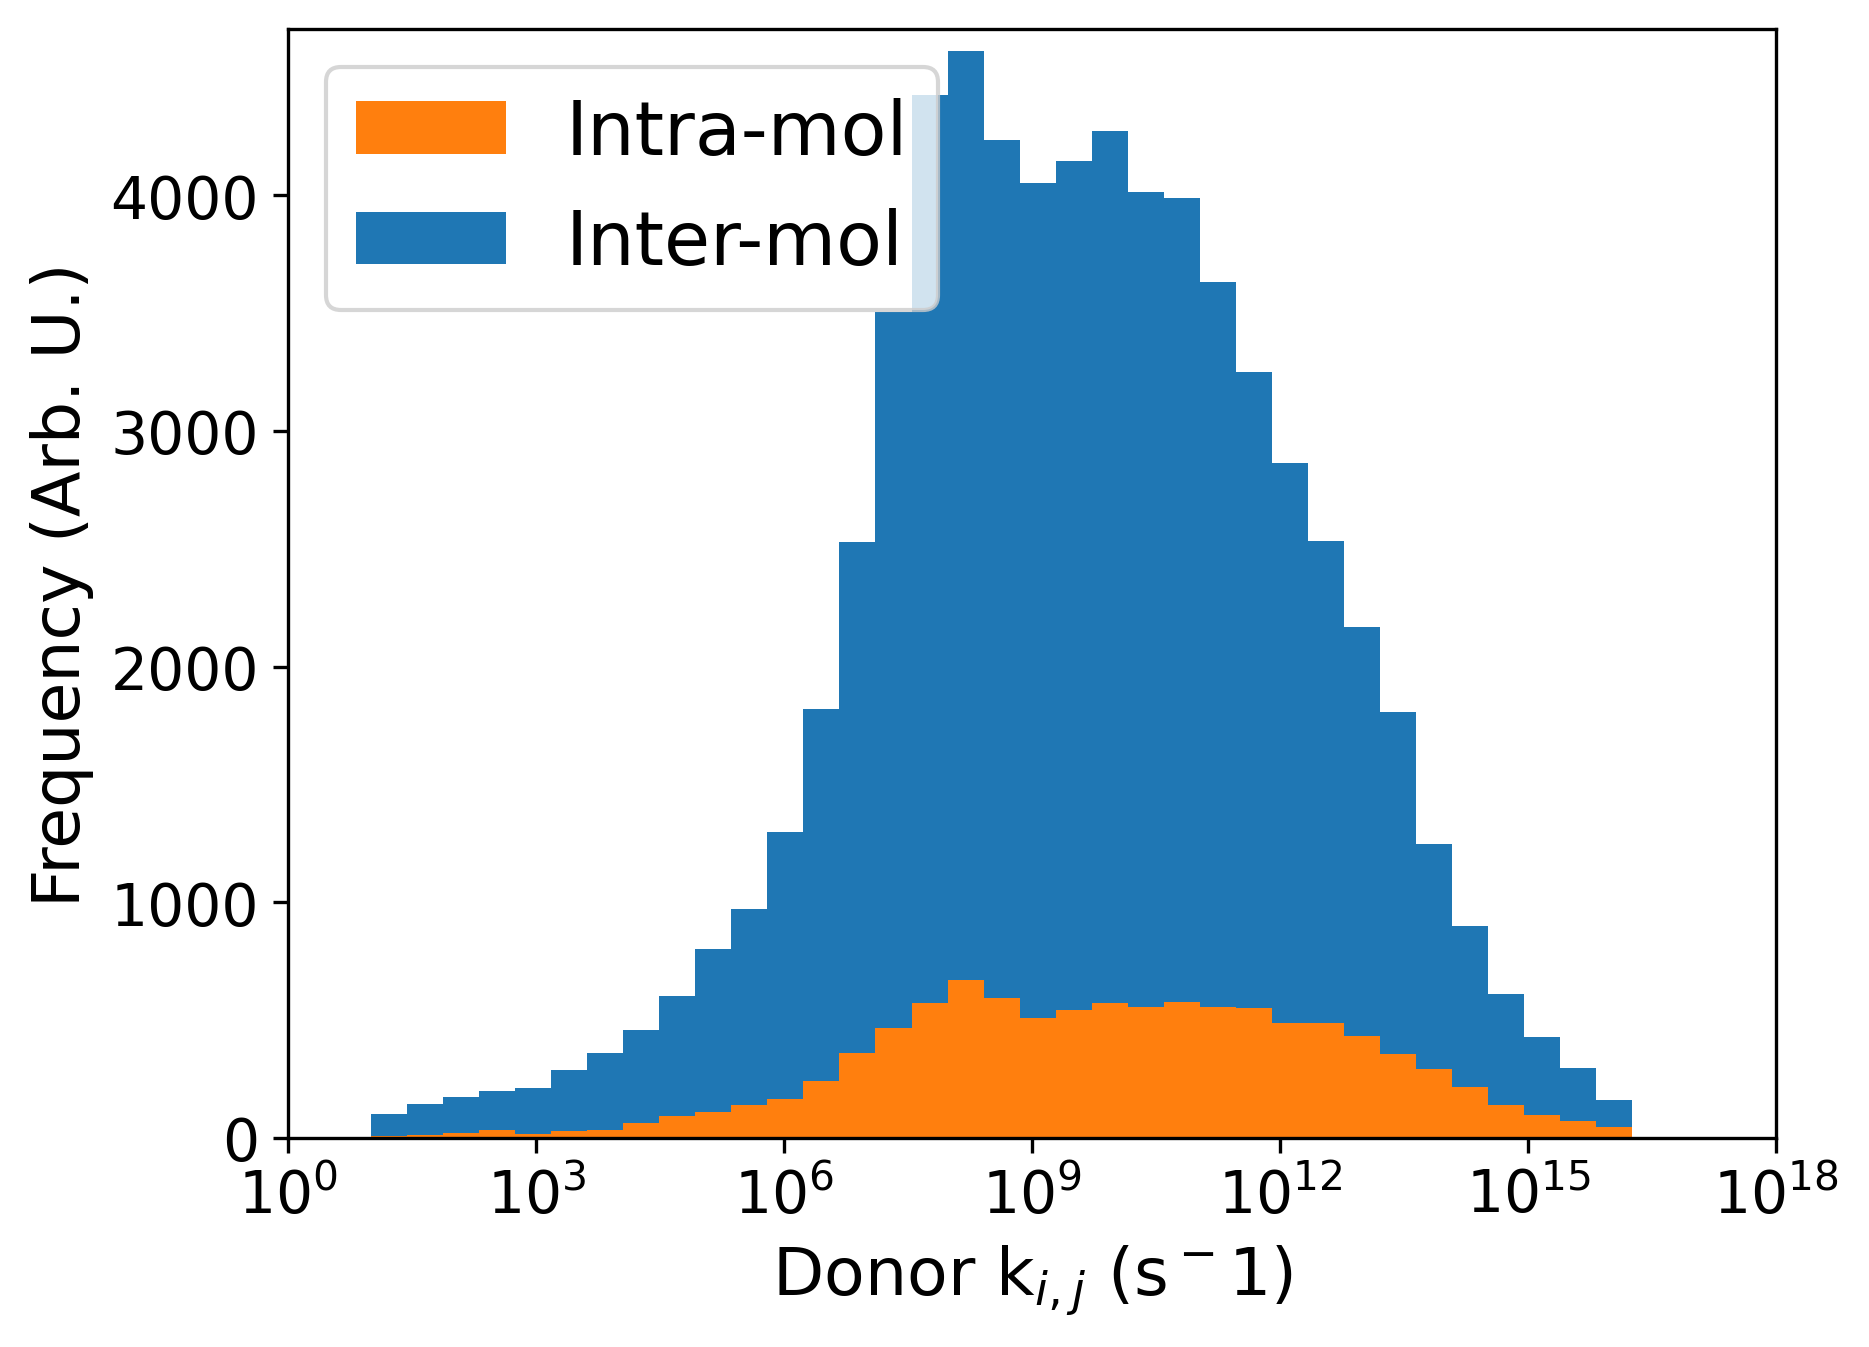
\includegraphics[width=\textwidth]{figures/donor_hopping_rate_clusters_temp100.png}
\end{subfigure}%
\begin{subfigure}{.5\textwidth}
    \textbf{(D) 800K}
    \centering
    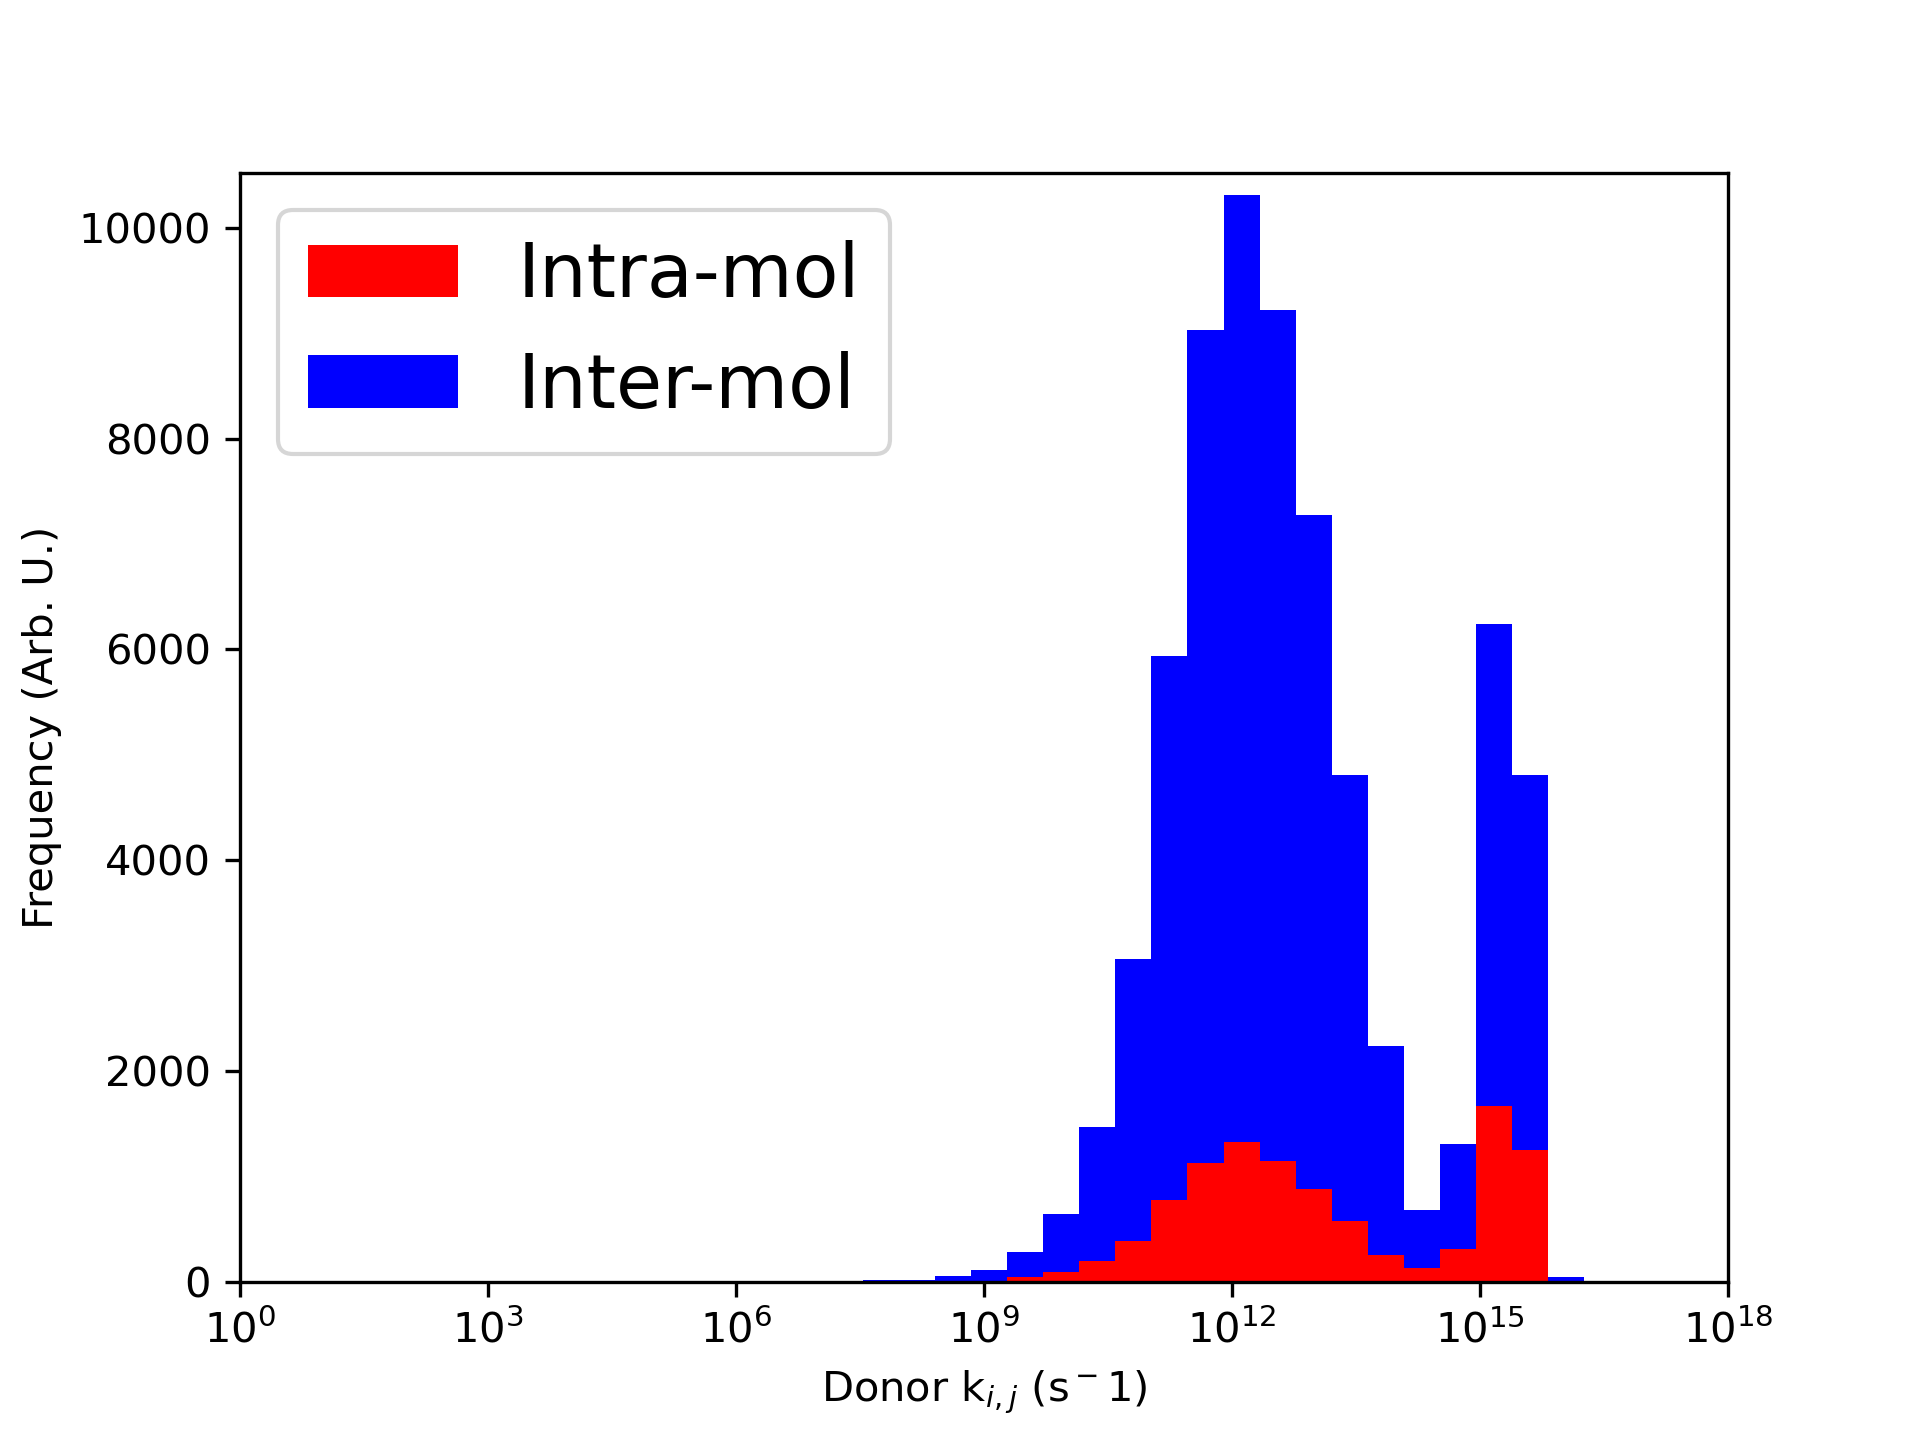
\includegraphics[width=\textwidth]{figures/donor_hopping_rate_clusters_temp800.png}
\end{subfigure}
\caption[short]{A beautiful, well written caption}
\label{TEMP}
\end{figure}

\subsection{MSD (lifetimes)}

The KMC algorithm allows an explicit calculation of the MSD accross a large number of 
particles in the system. Repeating along relevant time scales for 
charge transport, the slope of this relationship
can be estimated and related to to the 3D diffusion coeffiecient as discussed in the methods section of this
work. Mobility is obtained useing \autoref{einstein}, 
the groundwork for which Einstein derived in his doctoral dissertaion.

It is critical that we not include the ballistic transport timescale in the approximation of the limit
if the slope as time goes to infinity \cite{Maginn2018}. Estimating an upperbound for lifetimes such that
we can estimate the slope of the MSD as time goes to infinity can be messy. In real systems, free chrage
carrier lifetime is subject to a complex interplay between geminate recombination, non-geminate recombination,
charge trapping, temperature, and charge density, whose dynamics play out accros a picosecond to microsecond
timescales and vary widly form material to material as well as from microstrtucture to microstrucute for a
given material \cite{Laquai2015}.

For this work, the primary strategy was to avoid the ballistic region while exploring lifetimes
that are achievable computationally. For example, in an attempt to simulate out to the physical limit, a
simulation a microsecond($10^{-6}s$) lifetime resulted in a single hole hopping for 9 wall time hours.
It is advised that a preanalysis to determine where a given morphology's MSD will convergeb be performed so as
to never simulate past that point. Doing so is superflous and could introduce unessacery noise into the data. 

In the previous work on these P3HT morphologies, 7 liftimes were chosen and a linear regression was performed
to estimate the slope of the MSD. The current work found that the mobility can be apporpriately reproduced
with an appropriate choice of 2 lifetimes beyond the ballistic transport timescale. It was found that with the 
squared displacement averaged over 1000 holes at $10^{-9}s$ and again $10^{-10}s$ the slope of the MSD can be
commensurety reproduced with 1000's less individual holes having to be simulated. The results in the accuracy
section above were aquired with these 2 chosen lifetimes. I am currently running accross 7 lifetimes on the
crystalline morph. 

\begin{figure}
  \center
  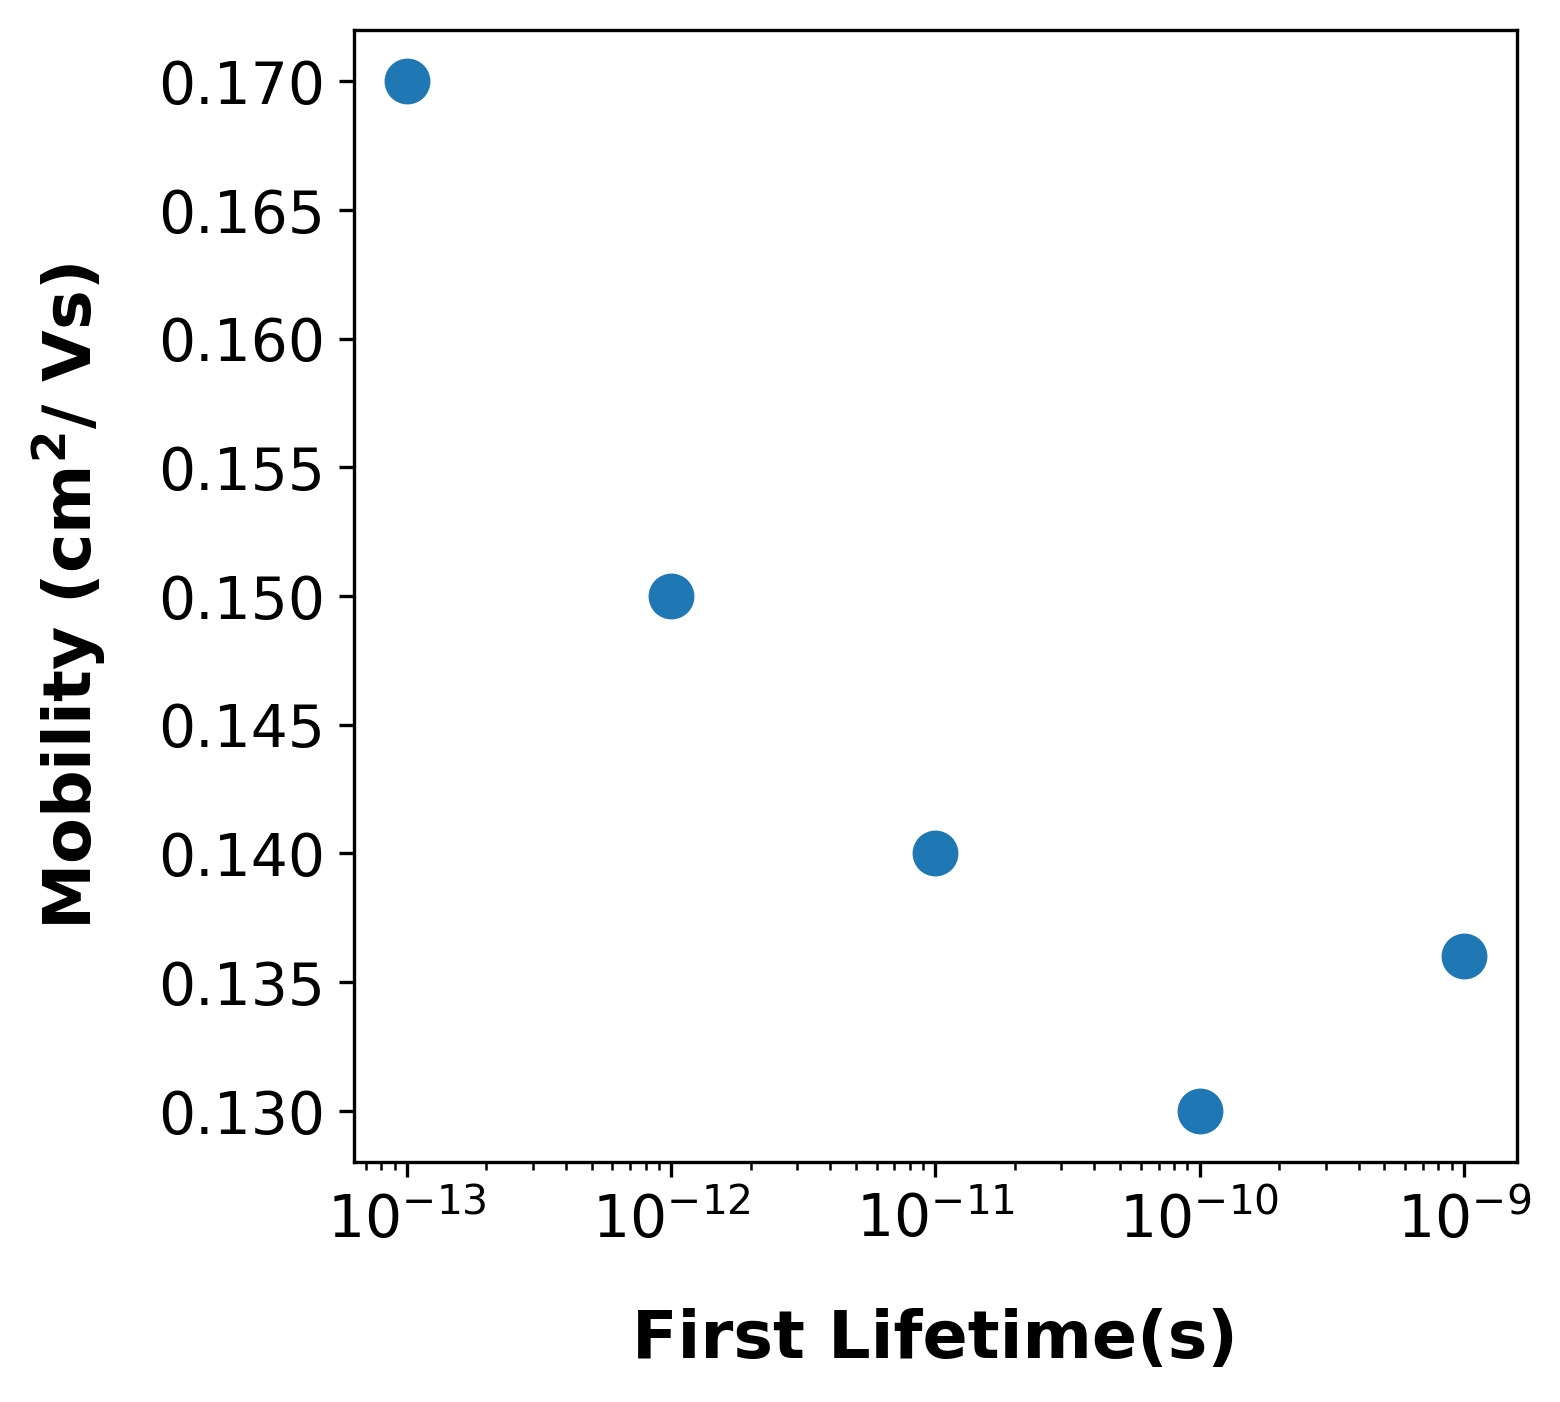
\includegraphics[width=0.8\linewidth]{figures/lifetime.png} 
    \caption{The results of running 5 KMC simulations with the first lifetimes as described in the text. It
    can be seen that below the the ballistic timescale (roughly $10^{-10}$), the resulting mobility is affected}
  \label{lifetime}
\end{figure}

With the slope between MSD at the first lifetime and at the second lifetime proving an estimate of the slope
of the MSD, 6 simulations we run with progressiveily shorter first lifetimes. That is, the second lifetime was
set to $10^{-8}s$ for all 5 simulations and the first lifetime was set to $10^{-9}s$, $10^{-10}s$,
$10^{-11}s$, $10^{-12}s$, and $10^{-13}s$ respectively. The results are plotted in figure
\ref{lifetime}. As expected, as the first lifetime progresses in the ballistic transport timescale, which this work
estimates around $10^{-10}s$, the resulting mobility increases. If the starting lifetime is even shorter the
workflow breaks down becuase as can be seen from the hop rate distribution in figure \ref{TEMP}(D), even at
extreme temperatures, holes need more time that that to hop even once. 

Interestingly, the algorithm seems to be quite robust against choice of lifetimes. As can be seen in the
figure, order of magnitude differences in lifetime choices results in less than 2X difference in the resulting
mobility. This further suggests that going lifetime crazy is a waste of computation.  

\section{ITIC}
\label{itic}
The ITIC morphology studied in \autoref{itic} was simulated using Plankton-Flow \cite{cmelab} on Fry,         
a high performance computing cluster at Boise State University.  
Using \texttt{planckton-flow}, a 1000
molecule morphology of ITIC was equillibrated over a 10e-7 step MD simulation at room temperature. 
From the results of the MD
simulation, the last frame of the atomic trajectories is taken to represent an accurate equillibrium geometry
of ITIC. 

To apply the hopping model to this atomistic morphology requires the
delineation of segments within the morphology upon which charges can delocalize along LUMO (or 
HOMO for donors). It should be noted that acceptor in this context doesn't refer to
chromophore $j$ as such.  
The LUMO of ITIC delocalizes along the backbone of the molecule, with
negligible electron density in the side chains and this makes the backbone of this kind of small molecule
material the obvious choice of chromophore.
. This has been quantified and well visualized using \textit{ab
initio} DFT at the level of the molecule by Han et al.~\cite{Han2019}.
We have visualized this at the nanometer scale in figure \ref{ITIC} using the openly
available visualization tool OVITO \cite{Stukowski2010a}. 
\begin{figure}
\centering
\begin{subfigure}{.5\textwidth}
    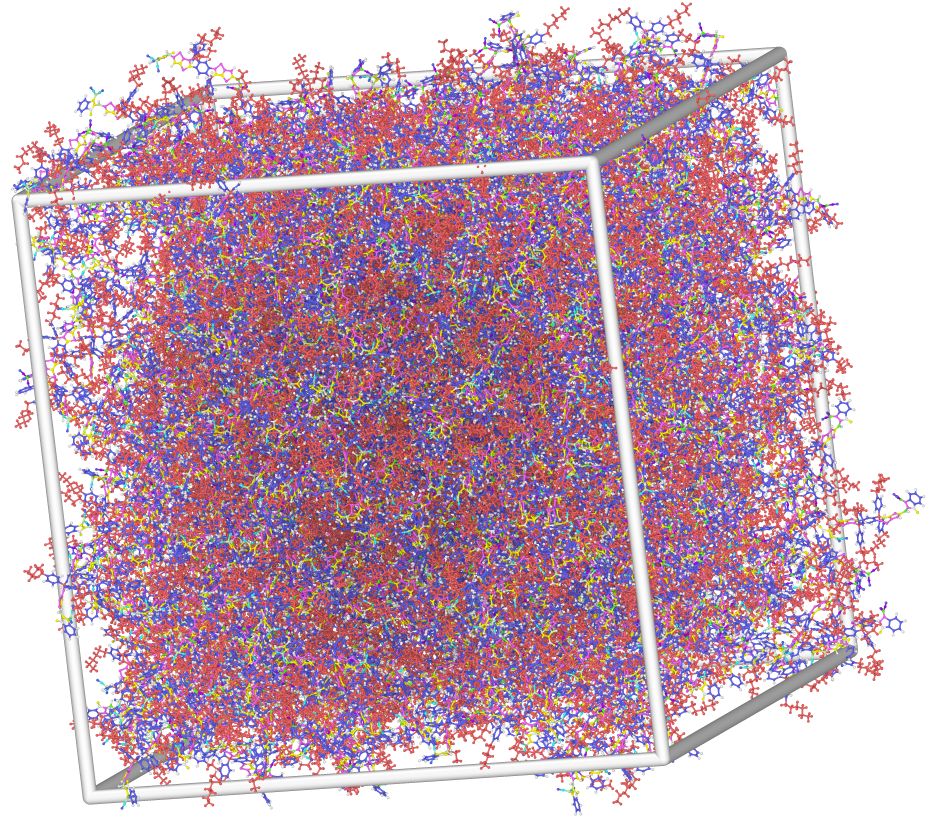
\includegraphics[width=\textwidth]{figures/ITIC-blackedout-unwrapped-allatom.png}
\end{subfigure}%
\begin{subfigure}{.5\textwidth}
    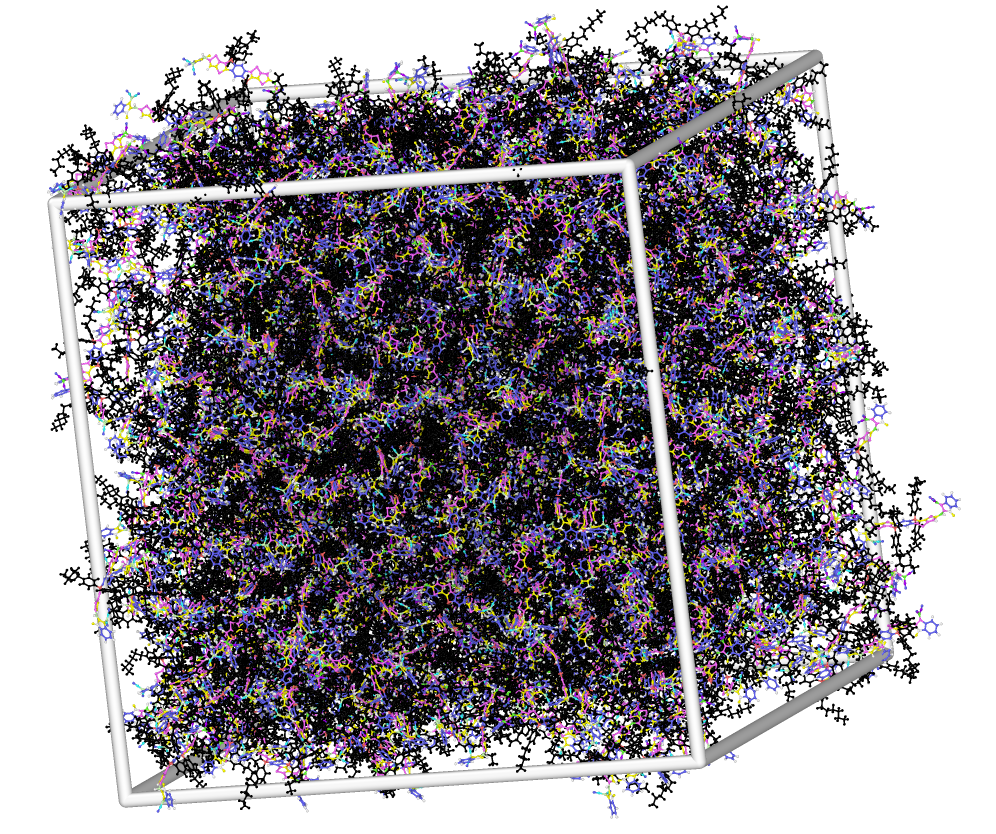
\includegraphics[width=\textwidth]{figures/ITIC-blackedout-unwrapped.png}
\end{subfigure}
    \caption[short]{1000 molecule ITIC morphology. Right: Segments known to participate in frontier
    molecular orbitals are in color and side chains in black.}
\label{ITIC}
\end{figure}

A single molecule ITIC has 186 atoms, with the backbone consisting of 70 atoms. We deployed two different
approaches to the delineation of chomophores within the ITIC morphology. In addition the the simulation of hopping
from backbone to backbone we ran simulations with the whole molecule prescibed as chromophores. This
necessarily requires more heavy lifting from \texttt{pySCF} but is trivially easy from an indexing perspective. Similar to the results of the DCUT
investigation, this implemenation of \texttt{pySCF} combined with clever pickling of system objects at various stages
of the workflow suggest that the laborious delineation of chromophores either via manual perscription or
by clever use of smarts matching is a fools errand. We found that, while the 70 atom chomophores took 1.2s
per dimer while the whole molecule dimer calculations with 186 atoms per chomophore to on average 3.3s.
Comprable mobilities of $(1.019 \pm 0.001)\cdot 10^{-3}$ or the backbone chromophores and 
$(1.275 \pm 0.001)\cdot 10^{-3}$ for the whole molecule. 
For small molecule materials this suggests forgoing labor intinsive indexing of chromophores.

As discussed in the sensitivity analysis, our mobility calcualtions are relatively sensitive to the choice of
reorganization energy. For ITIC, $\lambda_{internal}$ has been well investigated and is widely reported as
$~0.15eV$. The external reorganization is harder to estimate. We take $\lambda_{total}=0.3eV$ as we did for
P3HT. With the fused
backbone resulting in a higher internal contribution and the lack of long range order resulting in a lower
external contribution. 

The the reported
experimental electron mobility of ITIC varies depending on how it was processed and how it was measured. 
Time-of-flight electron mobilities on the order of $10^{-4}$ \cite{Mica2018} and field effect mobilities on the order of
$10^{-2}$ \cite{Park2018} have been reported. 


%%% Local Variables: 
%%% mode: latex
%%% TeX-master: "BSUmain"
%%% End: 
